%%%%%%%%%%%%%%%%%%%%%%%%%%%%%%%%%%%%%%%%%
% Masters/Doctoral Thesis 
% LaTeX Template
% Version 2.5 (27/8/17)
%
% This template was downloaded from:
% http://www.LaTeXTemplates.com
%
% Version 2.x major modifications by:
% Vel (vel@latextemplates.com)
%
% This template is based on a template by:
% Steve Gunn (http://users.ecs.soton.ac.uk/srg/softwaretools/document/templates/)
% Sunil Patel (http://www.sunilpatel.co.uk/thesis-template/)
%
% Template license:
% CC BY-NC-SA 3.0 (http://creativecommons.org/licenses/by-nc-sa/3.0/)
%
%%%%%%%%%%%%%%%%%%%%%%%%%%%%%%%%%%%%%%%%%

%----------------------------------------------------------------------------------------
%	PACKAGES AND OTHER DOCUMENT CONFIGURATIONS
%----------------------------------------------------------------------------------------

\documentclass[
11pt, % The default document font size, options: 10pt, 11pt, 12pt
%oneside, % Two side (alternating margins) for binding by default, uncomment to switch to one side
english, % ngerman for German
singlespacing, % Single line spacing, alternatives: onehalfspacing or doublespacing
%draft, % Uncomment to enable draft mode (no pictures, no links, overfull hboxes indicated)
%nolistspacing, % If the document is onehalfspacing or doublespacing, uncomment this to set spacing in lists to single
%liststotoc, % Uncomment to add the list of figures/tables/etc to the table of contents
%toctotoc, % Uncomment to add the main table of contents to the table of contents
%parskip, % Uncomment to add space between paragraphs
%nohyperref, % Uncomment to not load the hyperref package
headsepline, % Uncomment to get a line under the header
%chapterinoneline, % Uncomment to place the chapter title next to the number on one line
%consistentlayout, % Uncomment to change the layout of the declaration, abstract and acknowledgements pages to match the default layout
]{MastersDoctoralThesis} % The class file specifying the document structure

\usepackage[utf8]{inputenc} % Required for inputting international characters
\usepackage[T1]{fontenc} % Output font encoding for international characters
\usepackage{subcaption}
\usepackage{mathpazo} % Use the Palatino font by default
\usepackage{listings}

\usepackage[backend=bibtex,style=authoryear,natbib=true]{biblatex} % Use the bibtex backend with the authoryear citation style (which resembles APA)

\addbibresource{refs.bib} % The filename of the bibliography

\usepackage[autostyle=true]{csquotes} % Required to generate language-dependent quotes in the bibliography

\usepackage[draft]{todonotes}   % notes showed}

\usepackage{xcolor}
\colorlet{punct}{red!60!black}
\definecolor{background}{HTML}{FFFFFF}
\definecolor{delim}{RGB}{20,105,176}
\colorlet{numb}{magenta!60!black}

\lstdefinelanguage{json}{
    basicstyle=\normalfont\ttfamily,
    numbers=left,
    numberstyle=\scriptsize,
    stepnumber=1,
    numbersep=8pt,
    showstringspaces=false,
    breaklines=true,
    frame=lines,
    backgroundcolor=\color{background},
    literate=
     *{0}{{{\color{numb}0}}}{1}
      {1}{{{\color{numb}1}}}{1}
      {2}{{{\color{numb}2}}}{1}
      {3}{{{\color{numb}3}}}{1}
      {4}{{{\color{numb}4}}}{1}
      {5}{{{\color{numb}5}}}{1}
      {6}{{{\color{numb}6}}}{1}
      {7}{{{\color{numb}7}}}{1}
      {8}{{{\color{numb}8}}}{1}
      {9}{{{\color{numb}9}}}{1}
      {:}{{{\color{punct}{:}}}}{1}
      {,}{{{\color{punct}{,}}}}{1}
      {\{}{{{\color{delim}{\{}}}}{1}
      {\}}{{{\color{delim}{\}}}}}{1}
      {[}{{{\color{delim}{[}}}}{1}
      {]}{{{\color{delim}{]}}}}{1},
}

%\usep

%----------------------------------------------------------------------------------------
%	MARGIN SETTINGS
%----------------------------------------------------------------------------------------

\geometry{
	paper=a4paper, % Change to letterpaper for US letter
	inner=2.5cm, % Inner margin
	outer=3.8cm, % Outer margin
	bindingoffset=.5cm, % Binding offset
	top=1.5cm, % Top margin
	bottom=1.5cm, % Bottom margin
	%showframe, % Uncomment to show how the type block is set on the page
}

\lstset{
  language=bash,
  frame=top,frame=bottom,
  basicstyle=\small\normalfont\sffamily,    % the size of the fonts that are used for the code
  stepnumber=1,                           % the step between two line-numbers. If it is 1 each line will be numbered
  numbersep=10pt,                         % how far the line-numbers are from the code
  tabsize=2,                              % tab size in blank spaces
  extendedchars=true,                     %
  breaklines=true,                        % sets automatic line breaking
  captionpos=t,                           % sets the caption-position to top
  mathescape=true,
  stringstyle=\color{white}\ttfamily, % Farbe der String
  showspaces=false,           % Leerzeichen anzeigen ?
  showtabs=false,             % Tabs anzeigen ?
  xleftmargin=17pt,
  framexleftmargin=17pt,
  framexrightmargin=17pt,
  framexbottommargin=5pt,
  framextopmargin=5pt,
  showstringspaces=false      % Leerzeichen in Strings anzeigen ?
}


%----------------------------------------------------------------------------------------
%	THESIS INFORMATION
%----------------------------------------------------------------------------------------

\thesistitle{Thesis Title} % Your thesis title, this is used in the title and abstract, print it elsewhere with \ttitle
\supervisor{Dr. James \textsc{Smith}} % Your supervisor's name, this is used in the title page, print it elsewhere with \supname
\examiner{} % Your examiner's name, this is not currently used anywhere in the template, print it elsewhere with \examname
\degree{Doctor of Philosophy} % Your degree name, this is used in the title page and abstract, print it elsewhere with \degreename
\author{John \textsc{Smith}} % Your name, this is used in the title page and abstract, print it elsewhere with \authorname
\addresses{} % Your address, this is not currently used anywhere in the template, print it elsewhere with \addressname

\subject{Biological Sciences} % Your subject area, this is not currently used anywhere in the template, print it elsewhere with \subjectname
\keywords{} % Keywords for your thesis, this is not currently used anywhere in the template, print it elsewhere with \keywordnames
\university{\href{http://www.university.com}{University Name}} % Your university's name and URL, this is used in the title page and abstract, print it elsewhere with \univname
\department{\href{http://department.university.com}{Department or School Name}} % Your department's name and URL, this is used in the title page and abstract, print it elsewhere with \deptname
\group{\href{http://researchgroup.university.com}{Research Group Name}} % Your research group's name and URL, this is used in the title page, print it elsewhere with \groupname
\faculty{\href{http://faculty.university.com}{Faculty Name}} % Your faculty's name and URL, this is used in the title page and abstract, print it elsewhere with \facname

\AtBeginDocument{
\hypersetup{pdftitle=\ttitle} % Set the PDF's title to your title
\hypersetup{pdfauthor=\authorname} % Set the PDF's author to your name
\hypersetup{pdfkeywords=\keywordnames} % Set the PDF's keywords to your keywords
}

\begin{document}

\frontmatter % Use roman page numbering style (i, ii, iii, iv...) for the pre-content pages

\pagestyle{plain} % Default to the plain heading style until the thesis style is called for the body content

%----------------------------------------------------------------------------------------
%	TITLE PAGE
%----------------------------------------------------------------------------------------

\begin{titlepage}
\begin{center}

\vspace*{.06\textheight}
{\scshape\LARGE \univname\par}\vspace{1.5cm} % University name
\textsc{\Large Doctoral Thesis}\\[0.5cm] % Thesis type

\HRule \\[0.4cm] % Horizontal line
{\huge \bfseries \ttitle\par}\vspace{0.4cm} % Thesis title
\HRule \\[1.5cm] % Horizontal line
 
\begin{minipage}[t]{0.4\textwidth}
\begin{flushleft} \large
\emph{Author:}\\
\href{http://www.johnsmith.com}{\authorname} % Author name - remove the \href bracket to remove the link
\end{flushleft}
\end{minipage}
\begin{minipage}[t]{0.4\textwidth}
\begin{flushright} \large
\emph{Supervisor:} \\
\href{http://www.jamessmith.com}{\supname} % Supervisor name - remove the \href bracket to remove the link  
\end{flushright}
\end{minipage}\\[3cm]
 
\vfill

\large \textit{A thesis submitted in fulfillment of the requirements\\ for the degree of \degreename}\\[0.3cm] % University requirement text
\textit{in the}\\[0.4cm]
\groupname\\\deptname\\[2cm] % Research group name and department name
 
\vfill

{\large \today}\\[4cm] % Date
%\includegraphics{Logo} % University/department logo - uncomment to place it
 
\vfill
\end{center}
\end{titlepage}

%----------------------------------------------------------------------------------------
%	DECLARATION PAGE
%----------------------------------------------------------------------------------------

\begin{declaration}
\addchaptertocentry{\authorshipname} % Add the declaration to the table of contents
\noindent I, \authorname, declare that this thesis titled, \enquote{\ttitle} and the work presented in it are my own. I confirm that:

\begin{itemize} 
\item This work was done wholly or mainly while in candidature for a research degree at this University.
\item Where any part of this thesis has previously been submitted for a degree or any other qualification at this University or any other institution, this has been clearly stated.
\item Where I have consulted the published work of others, this is always clearly attributed.
\item Where I have quoted from the work of others, the source is always given. With the exception of such quotations, this thesis is entirely my own work.
\item I have acknowledged all main sources of help.
\item Where the thesis is based on work done by myself jointly with others, I have made clear exactly what was done by others and what I have contributed myself.\\
\end{itemize}
 
\noindent Signed:\\
\rule[0.5em]{25em}{0.5pt} % This prints a line for the signature
 
\noindent Date:\\
\rule[0.5em]{25em}{0.5pt} % This prints a line to write the date
\end{declaration}

\cleardoublepage

%----------------------------------------------------------------------------------------
%	QUOTATION PAGE
%----------------------------------------------------------------------------------------

\vspace*{0.2\textheight}

\noindent\enquote{\itshape Thanks to my solid academic training, today I can write hundreds of words on virtually any topic without possessing a shred of information, which is how I got a good job in journalism.}\bigbreak

\hfill Dave Barry

%----------------------------------------------------------------------------------------
%	ABSTRACT PAGE
%----------------------------------------------------------------------------------------

\begin{abstract}
\addchaptertocentry{\abstractname} % Add the abstract to the table of contents
The Thesis Abstract is written here (and usually kept to just this page). The page is kept centered vertically so can expand into the blank space above the title too\ldots
\end{abstract}

%----------------------------------------------------------------------------------------
%	ACKNOWLEDGEMENTS
%----------------------------------------------------------------------------------------

\begin{acknowledgements}
\addchaptertocentry{\acknowledgementname} % Add the acknowledgements to the table of contents
The acknowledgments and the people to thank go here, don't forget to include your project advisor\ldots
\end{acknowledgements}

%----------------------------------------------------------------------------------------
%	LIST OF CONTENTS/FIGURES/TABLES PAGES
%----------------------------------------------------------------------------------------

\tableofcontents % Prints the main table of contents

\listoffigures % Prints the list of figures

\listoftables % Prints the list of tables

%----------------------------------------------------------------------------------------
%	ABBREVIATIONS
%----------------------------------------------------------------------------------------

\begin{abbreviations}{ll} % Include a list of abbreviations (a table of two columns)

\textbf{LAH} & \textbf{L}ist \textbf{A}bbreviations \textbf{H}ere\\
\textbf{WSF} & \textbf{W}hat (it) \textbf{S}tands \textbf{F}or\\

\end{abbreviations}




%----------------------------------------------------------------------------------------
%	DEDICATION
%----------------------------------------------------------------------------------------

\dedicatory{For/Dedicated to/To my\ldots} 

%----------------------------------------------------------------------------------------
%	THESIS CONTENT - CHAPTERS
%----------------------------------------------------------------------------------------

\mainmatter % Begin numeric (1,2,3...) page numbering

\pagestyle{thesis} % Return the page headers back to the "thesis" style

% Include the chapters of the thesis as separate files from the Chapters folder
% Uncomment the lines as you write the chapters

% Chapter 1

\chapter{Introducción} % Main chapter title

\label{Chapter1} % For referencing the chapter elsewhere, use \ref{Chapter1} 

%----------------------------------------------------------------------------------------

% Define some commands to keep the formatting separated from the content 
\newcommand{\keyword}[1]{\textbf{#1}}
\newcommand{\tabhead}[1]{\textbf{#1}}
\newcommand{\code}[1]{\texttt{#1}}
\newcommand{\file}[1]{\texttt{\bfseries#1}}
\newcommand{\option}[1]{\texttt{\itshape#1}}

%----------------------------------------------------------------------------------------
\section{Abstract}

La reproducibilidad de experimentos es la habilidad de correr un experimento con la introducción de cambiar y obtener resultados que son consistentes con los originales. Para permitir la reproducibilidad, la comunidad científica ha incentivado a los investigadores a publicar la descripción de los experimentos.

%Experiment reproducibility is the ability to run an experiment with the introduction of changes to it and getting results that are consistent with the original ones. To allow reproducibility, the scientific community encourages researchers to publish descriptions of the these experiments. 

Sin embargo, estas recomendaciones no incluyen una forma automática para crear esta 
%However, these recommendations do not include an automated way for creating such descriptions: normally scientists have to annotate their experiments in a semi automated way. Moreover
In this paper we propose a system to automatically describe computational environments used in in-silico experiments. We propose to use Operating System (OS) virtualization (containerization) for distributing software experiments throughout software images and an annotation system that will allow to describe these software images. The images are a minimal version of an OS (container) that allow the deployment of multiple isolated software packages within it. 
Then we apply this approach over different real workflow and 
systems.

Experiment results shows that our approach can reproduce a equivalent environment using Docker Containers.
%----------------------------------------------------------------------------------------
%	SECTION 1
%----------------------------------------------------------------------------------------

\section{Experimentos científicos computacionales} 


El incremento de uso de las ciencias de la computación, que es la cien

El uso de la computación en la ciencia,



%context
The emergence of computational science, that is, science executed using computational models and simulations, has also implied an increasing interest on reproducibility

La reproducibilidad de experimentos es la habilidad de correr un experimento con la introducción de cambios y obtener resultados que son consistentes con los originales. La introducción de cambios permite evaluar diferentes características del experi




Experiment reproducibility is the ability to run an experiment with the introduction of changes to it and getting results that are consistent with the original ones. Introducing changes allows to evaluate different experimental features of that experiment since researchers can incrementally modify it, improving and repurposing the experimental methods and conditions~\cite{stodden2010reproducible}.
To allow experiment reproducibility it is necessary to provide enough information about that experiment, allowing to understand, evaluate and build it again. Usually, experiments are described in scientific workflows (representations that allow managing large scale computations) which run on distributed computing systems. 
To allow reproducibility of these scientific workflows it is necessary first to address a workflow conservation problem, since experimental workflows need to guarantee that there is enough information about the experiments so it is possible to build them again by a third party, replicating its results without any additional information from the original author~\cite{garijo2013quantifying}. 

To achieve conservation the research community has focused on conserving workflow executions by conserving data, code, and the workflow description, but not the underlying infrastructure (i.e. computational resources and software components). There are some approaches that that focused on conserving the environment of an experiment such as the work in~\cite{santana2017reproducibility} or the Timbus project\footnote{\url{http://www.timbusproject.net/}}~\cite{dappert2013describing} that focuses on business processes and the underlying software and hardware infrastructure. 

The authors in~\cite{santana2017reproducibility} identified two approaches for conserving the environment of a scientific experiment: physical conservation, where the research objects within the experiment are conserved in a virtual environment; and logical conservation, where the main capabilities of resources in the environment are described using semantic vocabularies to allow a researcher to reproduce an equivalent setting. The authors defined a process for documenting the workflow application and its related management system, as well as their dependencies. However this process is done in a semi-automated manner, leaving much work left to the scientists. Furthermore, usually most works leave out of the scope the physical conservation of the execution of scientific workflows. 

%need
However, logical and physical conservation are important to achieve the goals of the researchers.

La conversación lógica permite describir los recursos computaciones y a partir de estas descripciones cualquier cientifico podrá reconstruir la infraestructura y correr el experimento cíentifico. No obstante, el proceso de descripción debe ser automatico para evitar errores y perdidas de tiempo.

%will be able to reconstruct the infrastructure and run the experimient.

Y la conservación física permite distribuir fácilmente el ambiente computacional del workflow, evitando que los científicos hagan la configuración o la instalación de bibliotecas o binarios requeridas para ejecutarlo. Sin embargo, los trabajos anteriores muestran que la conservación física presentan dificultades debido al tamaño de la imagen que contiene el sistema operativo o 
Also, the main problem for conserving the physical environment of an experiment is the amount of space needed.



%task
Herein we propose a solution to improve the physical and logical conservation solution by using operating-system-level virtualization. This technology, also known as containerization, refers to an Operating System (OS) feature in which the OS kernel allows the existence of multiple isolated user-space instances called containers. 

One of the most popular virtualization technologies is Docker\footnote{\url{https://www.docker.com/}}, which implements software virtualization by creating minimal versions of a base operating system (a container). 
Docker Containers can be seen as lightweight virtual machines that allow the assembling of a computational environment, including all necessary dependencies, e.g., libraries, configuration, code and data needed, among others. 
Using Docker, the users can distribute these computational environments through software images. 


% With container virtualization it is possible to reduce to the minimum the size of the virtual machine needed for running the scientific workflow. 

We propose first to use Docker images as means for preserving the physical environment of an experiment. We use containers since they are lightweight and more importantly, they are easier to automatically describe so we  improve the process of documenting scientific workflows
In order to achieve logical conservation, we built a annotator system for the Docker Images that describe the workflow management system, as well their dependencies by developing an annotator system for the Docker images before.


%object
This work report the...


%%%%%%%%%%%%%%%%%%%%%%%%%%%%%%%%%%%%%%%%%%%%%%%%
%findings

%conclusion




\subsection{Experimental Sciences Approaches}

\subsubsection{In Vivo and In Vitro Science}

\subsubsection{In Silico Science}

\subsubsection{The Challenge of Scientific Reproducibility}


\subsection{Computational Scientific Experiments}

\subsubsection{Workflows in Science}


\subsection{Scientific Conservation and Reproducibility}

% Chapter 1

\chapter{Estado del arte} % Main chapter title

\label{Chapter2} % For referencing the chapter elsewhere, use \ref{Chapter1}


\section{Experimentos científicos computacionales} 

La reproducibilidad de los resultados en experimentos es una piedra angular del método científico. Es por ello, que la comunidad científica ha incentivado a los investigadores a publicar sus contribuciones en un forma verificable y entendible \cite{james2014standing,stodden2010reproducible}.

Los términos de reproducibilidad y repetibilidad son utilizados como sinónimos. En este trabajo, utilizaremos las definiciones propuestas por \cite{santana2017reproducibility}, replicabilidad será definida como recreación estricta del experimento original y reproducibilidad es menos restrictivo e implica que puedan existen algunos cambios.

Particularmente, en las áreas de la ciencia donde se ejecutan experimentos in-silico, o sea que realizan a través de computadores o simulaciones, la reproducibilidad requiere que los investigadores compartan el código y los datos de los experimentos realizados con el fin de que tanto los resultados como el método pueden ser analizados en una forma similar al trabajo original descrito en la publicación asociada a dicho experimento. Para lograr ese objetivo, el código debe estar disponible y los datos deben encontrarse en un formato leíble \cite{stodden2014implementing}.


\subsection{Conservación de procedimiento científicos}

Distintas áreas de la ciencia ha adoptado los workflows para conservar el procedimiento. Los workflows científicos son métodos que permiten representar un conjunto de pasos computacionales. Estos pasos pueden ser la obtención de los datos de entrada, transformaciones o generación de los resultados.
Por ejemplo, investigadores en bio-informática ha incorporado los workflows para distintos análisis: 
Doblamiento de proteínas \cite{craddock2006science}, secuencias de DNA y RNA \cite{blankenberg2010galaxy,giardine2005galaxy} y la detección de ondas gravitacionales \cite{deelman2004pegasus}.


La representación de los workflow se construye en un lenguaje abstracto para simplificar la complejidad. El conjunto de pasos se pueden representar como gráfos sin ciclos y dirigidos, donde cada paso computacional es representado por un nodo y las dependencias entre los pasos son representado por los arcos.

El uso de sistemas de manejo de workflows científicos \textit{Scientific Workflow management Systems (WMS)} ha sido adoptado por la comunidad permitiendo diseñar abstractamente y ejecutar el procedimiento científicos. 

Múltiples estudios han mostrado las dificultades reproducir los resultados de los experimentos: 






Dado que los workflows formalmente describen la secuencia de tareas computacionales y administración de datos, es fácil encontrar el camino de los datos producidos.
Un científico podría ver el workflow y los datos, seguir los pasos y llegar al mismo resultado. En otras palabras, la representación del workflow facilita la creación y administración de la computación y además construye una base en la cual los resultados pueden ser validados y compartidos.

Como se menciono, la mayoría de las propuestas de reproducibilidad de ambientes en las ciencias de computación se han enfocado en los datos, el código y la descripción de workflow pero ha dejando de lado los recursos computacionales y componentes de software. Siendo un recurso esencial para reproducir el experimento

De acuerdo a \cite{king1995replication}, en orden de reproducir o replicar un artefacto digital es necesario manejar su conservación y para alcanzar esta conservación se debe garantizar que: existe la suficiente información con la cual se pueda entender, evaluar y construir un trabajo anterior sin información adicional del autor. 

Uno de los trabajos que se ha enfocado en conservar los recursos de un ambiente computacional es \cite{santana2017reproducibility}. Donde los autores han identificado dos enfoques para conservar un ambiente científico. Conversación física: donde el objeto real es conservado dada la relevancia y la dificultada de obtener una replica y  Conversación lógica: donde los objetos son descriptos en una manera que un experimento similar puede ser obtenido en un futuro experimento.


\section{Sistemas de administración de workflows}

Cómo se menciono anteriormente, Los workflows científicos permiten a los usuarios expresar fácilmente tareas computacionales de varios pasos, por ejemplo, recuperar datos de un instrumento o una base de datos, reformatear los datos y ejecutar un análisis. 
Un flujo de trabajo científico describe las dependencias entre las tareas y en la mayoría de los casos el flujo de trabajo se describe como un gráfico acíclico dirigido (DAG), donde los nodos son tareas y los bordes denotan las dependencias de las tareas.
Una propiedad que define un flujo de trabajo científico es que gestiona el flujo de datos. Las tareas en un flujo de trabajo científico pueden ser de todo, desde tareas en serie cortas hasta tareas paralelas muy grandes (MPI, por ejemplo) rodeadas de un gran número de pequeñas tareas en serie utilizadas para el pre y postprocesamiento.
La interpretación y ejecución de los workflows son manejados por un sistema de manejo de workflows (WMS) que administra la ejecución de la aplicación en la infraestructura. 
Un WMS puede ser considerado como una capa intermedia necesaria para la abstracción y orquestación de prodecimiento científico. A continuación se describe algunos de los WMS más populares.

Actualmente, existen múltiples WMS que han sido generado por diversas comunidades.

\begin{description}
	\item [Galaxy:] Galaxy (Goecks et al., 2010) is a web-based WMS that aims to bring computational data analysis capabilities to non-expert users in the biological sciences domain. The main goals of the Galaxy framework are accessibility to biological computational capabilities and reproducibility of the analysis result by tracking the information related to every step on the process. 
	\item [Taverna: ] Taverna is a Web Service-based WMS, as all the components of the workflow must be implemented as web services (either locally or using an available remote service). Taverna is able to integrate Soaplab26, REST (Fielding, 2000) and WSDL (Christensen et al., 2001) web services. It offers a wide range of services for different processing capabilities, such as local Java services, statistical R processor services, XPath scripts, or spreadsheet import services.
	\item [Pegasus:] Pegasus (Deelman et al., 2005) is a WMS able to manage workflows comprised of mil- lions of tasks, recording data about the execution and intermediate results. In Pegasus, workflows are described as abstract workflows, which do not contain resource informa- tion, or the physical locations of data and executables.
	\item [WINGS:] WINGS (Gil et al., 2011) may not be considered as a proper WMS by itself, as it does not provide workflow enactment and execution features. However it is widely known for workflow design. WINGS can be seen as a top-level and domain-oriented design tool whose workflows can be later enacted in different workflow engines, such as Pegasus or Apache OODT29.
	\item [dispel4py:] dispel4py (Filguiera et al., 2014) is a Python (Rossum, 1995) library for describing workflows. It describes abstract workflows for data-intensive applications, which are later translated and enacted in distributed platforms (e.g. Apache Storm, MPI clusters, etc.).

\end{description} 

\subsection{Pegasus}

\subsection{Dispel4py}

\subsection{WINGS}

\section{Reproducibilidad en ciencias de la computación}

\subsection{Conservación de equipamiento}
El equipamiento en otras disciplinas comúnmente no es un problema a resolver dado que los recursos que se utilizan son son conocidos, no-variables y estándares. Por ejemplo, la utilización de probetas, microscopios u otros. Consecuentemente, son nombrados e identificado de forma manual en los procedimientos de los cuadernos de laboratorio. Lo que permite que otro investigador conozca cuáles fueron las herramientas utilizadas.
En otros casos como en biología, ciertos recursos son materiales y deben ser incluidos dentro de los procedimientos, esta información incluye marcas, composición y otra información. Y en la astronomía observamos  la utilización de recursos  de alta tecnología. donde también es necesario documentar las características de hardware y configuraciones utilizadas en el proceso experimental. 

En las ciencias de la computación observamos un caso similar, dado que los recursos computacionales son una componente en la ejecución del sistema. 
Es por ello, que los investigadores de esta comunidad que realizan publicaciones no debe ser la excepción respecto a la descripción de los recursos y los autores deben poder documentar computadores, clusters, servicios web, componentes de software, etc., en el contexto de sus experimentos.

En \cite{DBLP:conf/eScience/ZhaoGBKGGHRRG12} se estudia el factor de decaimiento de un set workflows científicos almacenado en myExperiment que fueron diseñados para el sistema Taverna del área de biología . Los autores utilizando cuatro conjuntos de paquetes de workflows y clasifican el decaimiento de los workflows en cuatro categorías: recursos de terceros volatiles, datos de ejemplos faltantes, ambiente de ejecución faltante y descripciones insuficientes sobre los workflow. El estudia muestra que casi el 80\% de workflows fallan al ser reproducidos, con un 12\% de esos fallos debido a ambiente de ejecución faltante y 50\% recursos de terceros volatiles.

En \cite{DBLP:conf/ipres/MatthewsCWJBS09}, los autores describen un procedimiento para preservar el software, argumentando que el software es frágil a los cambios de ambiente: hardware, sistema operativo, versiones de las dependencias y configuración. Los autores afirman que el software no puede ser preservado con la metodología de sólo mantener su código binario ejecutable y introducen el concepto de adecuación de la preservación, una métrica para medir si la preservación de conjunto de funcionalidades de componente de software luego de un proceso reproducción
La comunidad ha enfocado en mejorar los desafíos en la publicación de trabajos científicos, Elsevier formó el Executable Paper Grand Challenge para abordar el problema de que los resultados de la investigación informática pueden ser difíciles de reproducir. Los bloques vitales de información necesarios para replicar tales resultados -por ejemplo, software, código, grandes conjuntos de datos- no suelen estar disponibles en el contexto de una publicación académica.  Executable Paper Grand Challenge crea una oportunidad para que los científicos diseñen soluciones que capturen esta información y proporcionen una plataforma para que estos datos puedan ser verificados y manipulados. En 2011, \cite{DBLP:journals/procedia/BrammerCMW11} argumentaron que el documento de investigación en su estado actual ya no es suficiente para reproducir, validar o revisar completamente los resultados y conclusiones experimentales de un documento. Esto impide el progreso científico. Para remediar estas preocupaciones, presentan Paper Maché, un nuevo sistema para crear documentos de investigación dinámicos y ejecutables. La principal novedad de Paper Maché es el uso de máquinas virtuales, que permite a los lectores y revisores ver e interactuar fácilmente con un documento y reproducir los principales resultados experimentales.
En la misma línea, CernVM \cite{buncic2010cernvm} propuso la utilización de máquinas virtuales para resolver problemas de reproducibilidad en la ciencia. CernVM es un sistema para el uso de máquina virtuales capaz de ejecutar aplicaciones físicas de los experimentos del LHC en el CERN. Su objetivo es proporcionar un entorno completo y portátil para desarrollar y ejecutar el análisis de datos LHC en cualquier ordenador de usuario final (portátil, de sobremesa), así como en la red, independientemente de las plataformas de sistemas operativos (Linux, Windows, MacOS). La motivación del uso de técnicas de virtualización que permite separar los recursos de computación desde la infraestructura subyacente.

Algunos autores han expuesto la necesidad de capturar y preservar el entorno de ejecución de un ejecución del experimento, proporcionando herramientas para analizar y empaquetar los recursos involucrados en el mismo.
ReproZip \cite{DBLP:conf/tapp/ChirigatiSF13} busca captar el conocimiento sobre una infraestructura e intentar reproducirlo en un nuevo entorno. Esta herramienta lee los componentes de infraestructura involucrados en la ejecución (archivos, variables de entorno, etc.) y almacena esta información en una base de datos MongoDB \footnote{\url{https://www.mongodb.com/es}}. A continuación se recogen y empaquetan los elementos descritos. Luego, el sistema debe desempaquetar en otra máquina para repetir el experimento. Sin embargo, este tipo de enfoque que empaqueta los componentes físicos de una infraestructura determinada presenta limitación en la práctica, debido que los paquetes deben ser ejecutado en un máquina destino similar.
TOSCA (Topology and Orchestration Specification for Cloud Applications) es un ejemplo de soluciones que han definido sintaxis para describir la ejecución de los ambientes computacionales. TOSCA es un lenguaje de código abierto utilizado para describir las relaciones y dependencias entre servicios y aplicaciones que residen en una plataforma de computación en nube. TOSCA puede describir un servicio de computación en nube y sus componentes y documentar la forma en que están organizados y el proceso de orquestación necesario para utilizar o modificar dichos componentes y servicios. Esto proporciona a los administradores una forma común de gestionar aplicaciones y servicios en la nube, de modo que esas aplicaciones y servicios puedan ser portátiles a través de las diferentes plataformas de los proveedores de cloud computing. 
Otro esfuerzo importante relacionado a nuestro trabajo incluye la descripción de los ambientes computaciones utilizando ontologías es TIMBUS. El proyecto se focaliza en preservar procesos de negocios y su infraestructura computacional.  Para ello, propusieron un extractor para extraer y anotar los componentes de Software y Hardware, éstas anotaciones son almacenada según un conjunto de ontologías  para gestionar la preservación y reejecución de los procesos de negocio. Sin embargo, el enfoque extractor del Proyecto Timbus no es adecuado para ser utilizado en Contenedores ya que aumenta la complejidad del contenedor, exige ejecutar el sistema lo cual conlleva aumento del costo computacional y creación de brechas de seguridad. 


Los autores en \cite{santana2017reproducibility} identificaron dos enfoques para conservar el medio ambiente de un experimento científico: la conservación física, donde los objetos de investigación dentro del experimento se conservan en un entorno virtual; y la conservación lógica, donde las principales capacidades de los recursos en el entorno se describen utilizando vocabularios semánticos para permitir al investigador reproducir un entorno equivalente. Definieron un proceso para documentar la aplicación de flujo de trabajo y su sistema de gestión relacionado, así como sus dependencias. Además, los autores propusieron The Workflow Infrastructure Conservation Using Semantics ontology (WICUS). WICUS es una red de ontologías OWL2 (Web Ontology Language) que implementa la conceptualización de los principales dominios de una infraestructura computacional. Estos hijo: Hardware, Software, Workflow y Recursos Informáticos. El flujo de trabajo científico requiere una pila de componentes de software, y los investigadores deben saber cómo desplegar esta pila de software para lograr un entorno equivalente.
Sin embargo, este proceso se realiza de forma de manual, dejando mucho trabajo a los científicos. 

Los autores afirman que la conservación de los ambientes computacionales comúnmente se logra utilizando un enfoque físico, debido a que esto permite compartir fácilmente un ambiente computacional con otros investigadores y ellos pueden reproducir el experimento utilizando en el mismo ambiente. 
Sin embargo, los esfuerzos necesarios para mantener la infraestructura son altos y no hay garantías que no sufran un proceso de decaimiento \cite{DBLP:journals/fgcs/DeelmanVJRCMMCS15}.  
Consecuentemente, la mayoría de las trabajo dejan fuera del ámbito de aplicación la conservación física del entorno informático del flujo de trabajo (basándose en la infraestructura elegida). Sin embargo, la conservación lógica y física es importante para lograr la reproducibilidad del experimento. 

En diversos trabajos \cite{DBLP:journals/bioinformatics/LeprevostGARUBV17}, ~\cite{Beaulieu2017}, ~\cite{Boettiger:2015:IDR:2723872.2723882} y \cite{aranguren2015enhanced} se ha propuesto la utilización de Docker como un reemplazo al uso de máquina virtuales como ambiente computacionales científicos, los trabajos argumentan que Docker presenta beneficios de portalibilidad, documentación precisa de la instalación y configuración, manejo de control de versiones de las imágenes y fácil adopción. 
Un ejemplo de uso de Docker para la reproducibilidad es BioContainers \cite{DBLP:journals/bioinformatics/LeprevostGARUBV17} es un framework de código abierto y orientado a la comunidad que proporciona entornos ejecutables independientes de la plataforma para el software de bioinformática. BioContainers permite a los laboratorios instalar fácilmente software de bioinformática, mantener múltiples versiones del mismo software y combinar herramientas en poderosas tuberías de análisis. BioContainers se basa en los populares proyectos de código abierto Docker y rkt, que permiten que el software sea instalado y ejecutado bajo un entorno aislado y controlado.
Sin embargo, en \cite{Boettiger:2015:IDR:2723872.2723882,DBLP:conf/semweb/OsorioAV18} los autores exponen que Docker no controla que paquetes hay en las imágenes y no existe una descripción completa de los componentes del container. Así, las imágenes Docker funcionan como una caja negra, lo que significa que los usuarios saben que el paquete de software principal se ejecuta dentro del contenedor pero no conocen las versiones o los otros paquetes necesarios para ejecutarlo.

%caja negra
En \cite{Shu:2017:SSV:3029806.3029832:DockerHub:Security} analizó más de 300.000 imágenes de Docker almacenadas en el repositorio oficial de Docker. Los autores han encontrado en promedio que las imágenes que contiene el Docker Hub son más de 180 vulnerabilidades, siendo la raíz de tal cantidad de vulnerabilidades el hecho de que muchas imágenes no han sido actualizadas en varios días; muchas de estas vulnerabilidades se propagan de imágenes de padres a hijos. Los autores encontraron correlaciones entre las imágenes más influyentes y los paquetes vulnerables mejor clasificados, lo que sugiere que la fuente de esa cantidad de vulnerabilidades era probablemente el resultado de la propagación de un pequeño número de imágenes populares (debido a la falta de actualización de las imágenes principales). Los autores utilizaron el software Clair \footnote{\url{https://github.com/coreos/clair}} de la empresa CoreOS\footnote{\url{https://coreos.com/}}. 


En términos de ingeniería ontológica, los autores in~\cite{huo2015smart} presentan la ontología Smart Container que extiende DOLCE~\cite{gangemi2002sweetening} y modela Docker en términos de sus interacciones para desplegar imágenes. Otro trabajo relacionado, ~\cite{tommasini2017representing}  describe cómo usar RDF para representar archivos de construcción de Docker. 





\section{Docker Overview}



\label{sec-Docker_overview}
Docker is a technology that allows virtualizing a minimal version of an Operating System. Therefore users can run applications within it. Throughout this section, we introduce how Docker and its registry (Docker Hub) work, starting with how Docker images are created and stored in Docker Hub. 

\subsection{Docker repositories and files}

Docker builds a software image by reading a set of instructions from a Dockerfile. A Docker file is a text file that contains all commands to build a Docker image. Docker files usually have multiple lines, which are translated into image layers whereas Docker builds the image. In the build process, the command is executed sequentially, creating one layer after the other. When an image is updated or rebuilt, only modified layers (i.e., modified lines) are updated. 


\subsection{Publishing and Deploying Docker images from Docker Hub}

Docker Hub is an online registry that stores two types of public repositories, both official, and community. Official repositories contain public, verified images such as Canonical, Nginx, Red Hat, and Docker. At the same time, community repositories can be public or private and are created by any user or organization.
By using that registry and a command line, it is possible to download and deploy Docker images locally as a running container into a host executing thus the software within the image. 
Anyone has the chance to create and store images into the Docker Hub registry by first creating a descriptor file called Dockerfile. 
This descriptor describes what software packages will be within the image, builds the image and finally uploads it to Docker Hub. However, Docker Hub does not control what packages are in the images, whether the image will deploy correctly or the images might have any security problem. 
Thus, Docker images work as a black box, which refers that users know that the main software package runs within the container but they do not know the other packages needed to run it.



There are two ways of uploading images to a user repository, either by a push from a local host or automating that process from a Github repository. In order to push a repository to the Docker Hub, the users need to name their local images using their Docker Hub username, and the repository name they had created. Afterwards, users add multiple images to a repository by adding a specific \texttt{:<tag>} to it. This is all the information that normally Docker images have, being thus almost impossible to reproduce the execution environment if any of the used software packages within the images is modified. 

\section{Clair} 
% Chapter Template

\chapter{Objetivos de trabajo}

\label{Chapter3} 

El principal objetivo de este trabajo es complementar enfoques existentes para la reproducibilidad científica en el área de las ciencias de la computación. Para ello, se propone un nuevo enfoque para conservar el ambiente de ejecución del experimento científico.
Hemos identificado problemas abiertos, en orden de definir los objetivos de trabajo. Luego, estos objetivos se ven formalizados por un conjunto de hipótesis. Y además, se define un conjunto de hechos que se asumen para restringir el campo de aplicación de la propuesta.

%--------------------------------------------
%	SECTION OPEN RESEARCH PROBLEMS
%-------------------------------------------


\section{Open Research Problems}
\begin{itemize}
	\item Problema 1: La infraestructura computacional utilizada por un workflow científico se encuentra predefinida. Por lo tanto, no existe una definición de los recursos de la infraestructura para ejecutar el experimento. Consecuentemente, pueden existir dificultades para lograr la reproducción del experimento. 
	\item Problema 2: La conservación física de los ambientes computaciones permite mantener y compartir fácilmente el ambiente con la comunidad. Sin embargo, se ha descartado debido a tres problemas: 
		1. Alta utilización de almacenamiento por parte de las máquinas virtuales, 
		2. El acceso a los datos almacenados está sujetos a políticas de la organización 
		y 3. Existe un proceso de decaimiento en tiempo.
		Sin embargo, no se ha estudiado el uso de containers para solucionar el problema.
	\item Problema 3: Los enfoques actuales anotan los pasos de construcción de los ambientes computacionales de forma indirecta, por lo tanto, recaen en el científico 
\end{itemize}

%--------------------------------------------
%	SECTION HIPÓTESIS
%-------------------------------------------



\section{Hipótesis}

En función a los problemas abiertos detectados, se definen las siguientes hipótesis:

\begin{itemize}
	\item Un proceso automático puede describir los requerimientos de ambiente computacional y codificarlo en un formato compartible  utilizando modelos semánticos.
	\item La descripción de containers utilizando modelos semánticos permite la reproducción del ambiente de un experimento científico.
\end{itemize}
%--------------------------------------------
%	SECTION OBJETIVOS
%-------------------------------------------


\section{Objetivos}

Para enfrentar los problemas abiertos se definen los siguientes objetivos. Estos objetivos permiten la verificación de la hipótesis y ser una guía para el desarrollo.



\begin{itemize}
	\item Lograr conservación física y lógica de los ambientes computaciones de un experimento usando Containers
%	\item Conduct logical and physical conservation of the computational environment of the experiment using containers.
	\item Implementar un proceso automático capaz de leer la descripción del ambiente y especificar uno nuevo.
%	\item Implement an automated process able to read the mentioned information and specify a new environment of it, supporting the formerly required features.
	\item Integrar un sistema que permita el despliegue de estos ambientes computacionales en proveedores de infraestructura e instalar el software apropiado basado al plan de despliegue.
%	\item Integrate a system that allows the deployment of these computational environments in various infrastructure providers and install the appropriate software based on the deployment plan.

\end{itemize}
\subsection{Objetivos específicos}

\begin{itemize}
	\item Adaptar y mejorar modelos estándares que describen ambientes computacionales científicos para incluir virtualización basada en containers.
	\item Designar una framework para anotar los componentes de ambiente del experimento usando modelos semánticos.
%	\item 	Adapt and improve standard models that describe Computational Scientific Experiment to include Container-based virtualization.
%	\item Designate a framework to annotate the components of the environment’s experiments using the previous models.
\end{itemize}



\section{Restricciones}

\begin{itemize}
	\item Ambientes Linux
\end{itemize}
% Chapter Template

\chapter{Representación de ambiente de ejecución} % Main chapter title
%\section{Reproducibility in scientific workflows using Docker Containers} \label{s4}

%In this paper, we argue that the description of computational environments is necessary for the reproduction of the experiment. Furthermore, the information must be enough to compare and detect differences between the original and the reproduced environments.

En este trabajo, nosotros argumentamos que las descripciones de los ambientes computacionales es necesaria para la reproducción  del experimento. Además, la información debe ser la suficiente para comparar y detectar las diferencias entre el ambiente original y el reproducido.

Dada que las imágenes Docker son un ambiente aislada y independiente, los componentes de software dentro del container están relacionado al experimento y no existen componentes no relacionados. 
Por esta razón, nosotros aseguramos que las anotaciones no presentarán ruido de otras herramientas o dependencias asociadas.
Para realizar una anotación automática de los paquetes instalados, nosotros proponemos, e implementamos un sistema de anotación.
El sistema requiere el nombre de una imagen existente en un repositorio de DockerHub y opcionalmente los datos del repositorio Git que almacena el archivo Dockerfile. 

Los pasos asociados del sistema anotación:

\begin{enumerate}
	\item Consultar a repositorio los metadatos de la imagen. Anotar los metadatos utilizando la ontología propuesta.
	\item Descargar cada una de las capas asociadas a la imagen Docker.
	\item Utilizar Clair, Clair monta cada una de capas de la imagen, detecta los componentes de software instalados utilizando el sistema de paquete.
	\item Obtener la información de Clair, anotar los datos obtenidos por Clair según la ontología.
	\item Guardar los datos en una base de datos RDF que permita consulta SPARQL.
\end{enumerate} 

%----------------------------------
% 4.1 Semantic models
%----------------------------------
\section{Semantic models}\label{s4.1}
     
En \cite{santana2017reproducibility}, los autores proponen \emph{The Workflow Infrastructure Conservation Using Semantics ontology (WICUS)}. WICUS es ontología OWL2 (Web Ontology Language) que implementa la conceptualización de los principales dominios de la infraestructura computacional. Estas son: Hardware, Software, Workflow y recursos de computo
     
Los autores definen que los workflows cientificos requieren un conjunto de componentes de software, y los investigadores deben conocer como desplegar estos componentes para lograr ambiente equivalente.
Por lo tanto, nosotros utilizamos algunos clases y relaciones desde la ontología WICUS:

\begin{description}
	\item [DeploymentPlan:]  Un plan de despliegue está compuesto de todos los pasos  
	\item 
	El plan de despliegue permite entender al investigador cuáles fueron los pasos requeridos para construir el ambiente computacional.
	\item [DeploymentStep:] Cada paso de despliegue es representado por una línea de comando que realiza la instalación, descarga o configuración del ambiente. La información se obtiene desde el archivo DockerFile
	\item [ConfigurationInfo:]
	\item [ConfigurationParameter:]  
	\item [SoftwareStack:]
	\item [SoftwareComponent:]
\end{description} 


Definimos \verb|SoftwarePackage| como una subclase de \verb|SoftwareComponent| para definir los componentes instalados por el gestor de paquetes del sistema operativo y \verb|CondaPackage| los componentes instalados por el sistema de paquetes Conda.
Cada \verb|wicus:SoftwareComponent| tiene una relación \verb|dockerpedia:hasVersion| que muestra la versión del software instalado.

\todo[inline]{P4.1.2 Explicación de los cambios en la ontología}

Our final ontology is depicted in Figure~\ref{fig:ontology}. 

\begin{figure}
  \caption{Docker ontology.}
  \centering
    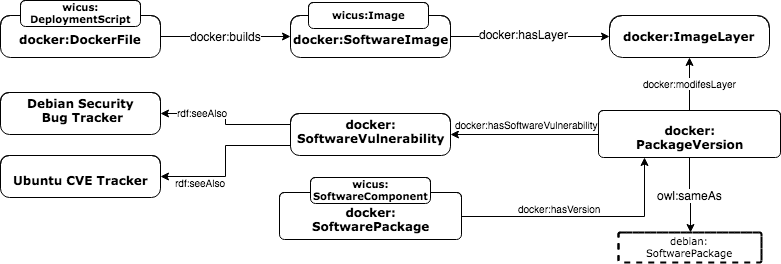
\includegraphics[width=0.4\textwidth]{Figures/dockerOntologyBasic.png}
    \label{fig:ontology}
\end{figure}



%----------------------
% 4.2 Annotator
%-----------------------
\section{Annotator}\label{s4.2}

%url de repositorio github y ubicación del Dockerfile
El servicio de anotación utiliza una interfaz REST para recibir la imagen Docker del experimento científico. Opcionalmente, el usuario puede entregar la información sobre el repositorio Git.  

 El sistema anotación realiza dos tipos de anotaciones: Componentes de software y pasos de construcción 

 
%--------------------------------------------
% 4.2.1 Building steps annotations
%---------------------------------------------
\subsection{Building steps annotations}\label{s4.2.1}

Anotamos el plan de despliegue (Deployment Plan) usando dos métodos. El primero método obtiene los pasos desde el archivo Dockerfile entregado por el usuario, esto permite obtener los pasos y la ubicación de archivo en el repositorio. 

Este método asegura la reconstrucción del ambiente debido a que cualquier archivo necesario por Dockerfile se encuentra en el repositorio Git.

Sin embargo, un usuario puede construir una imagen sin compartir el archivo Dockerfile. ~\cite{}. reporta que el 30\% de las imágenes Docker en DockerHub enlanza su archivo Dockerfile. 

Por lo tanto, nosotros extraemos la información utilizando el manifesto de la imagen Docker. Según la documentación de Docker, el manifiesto de la imagen provee la configuración y el conjunto de las capas de la imagen

Algunos atributos importantes son:

\begin{description}
	\item [name:] \textit{string} name is the name of the image’s repository
	\item [tag:] \textit{tag} is the tag of the image
	\item [architecture:] \textit{string} architecture is the host architecture on which this image is intended to run. This is for information purposes and not currently used by the engine
	\item [fsLayers:] \textit{array} fsLayers is a list of filesystem layer blob sums contained in this image. \\ 
		An fsLayer is a struct consisting of the following fields:
		\begin{description}
			\item [blobSum:] blobSum is the digest of the referenced filesystem image layer. A digest must be a sha256 hash
		\end{description}
	\item [history]: \textit{array} history is a list of unstructured historical data for v1 compatibility. It contains ID of the image layer and ID of the layer’s parent layers. A history is a struct consisting of the following fields:
	\begin{description}
		\item[v1Compatibility]:  \textit{string} V1Compatibility is the raw V1 compatibility information. This will contain the JSON object describing the V1 of this image. A V1Compatibility is a struct consisting of the following fields:
		
		\begin{description}
			\item [Id:] \textit{string} ID of the layer using sha256 hash
			\item [Parent:] \textit{string} ID of the parent layer using sha256 hash
			\item [ContainerConfig:] \textit{string} The command that built the layer
			\item [Author:] \textit{string} The name and email of the author
		\end{description}
	\end{description}
\end{description}

\todo[inline]{P4.3.3 Explicar como guardamos la información en RDF}


\todo[inline]{P4.3.4 Mostrar un ejemplo de anotación}

%--------------------------------------------
% 4.2.2 Software Components annotations
%---------------------------------------------
\subsection{Software Components annotations}\label{s4.2.2}


Nosotros lograr la anotación de los componentes de software utilizando los sistemas de paquetes del sistema, un sistema de paquete es una colección de herramientas de software que automatizan la instalación, actualización, configuración y eliminación de componentes de software. 
Clasificamos los sistemas que paquetes en dos tipos: sistemas de paquetes del sistemas y generales:

\begin{description}
	\item  [Sistemas de paquetes de sistema:] son aquellos vinculados al sistema operativo (e.g., apt de familia Debian, yum de familia RedHat).
	\item [Sistemas de paquetes generales:] son aquellos externos que normalmente son utilizados para instalar un componentes de software de tercero ó un lenguaje especifico (e.g., pip, conda, npm). Conda es un sistema paquete frecuentemente utilizado por investigadores al estar relacionado con Jupyter Notebook.

\end{description}

%We achieve the software components annotations using software package manager, a package manager system is a collection of software tools that automate the process of installing, upgrading, configuring, and removing software components. 

\subsection{Desafios}\label{s4.2.2}

La descripción de los componentes de software es fundamental para realizar cuantificar la similitud entre dos o más ambientes computacionales.
Un enfoque común para detectar los componentes de software guardar o detectar los comandos que realizan la instalación de software. Por ejemplo, la figure \ref{} muestra los comandos para instalar los componentes de la imagen TensorFlow. 


\begin{lstlisting}
apt-get install -y --no-install-recommends \
        build-essential \
        curl \
        libfreetype6-dev \
        libhdf5-serial-dev \
        libpng12-dev \
        libzmq3-dev \
        pkg-config \
        python \
        python-dev \
        rsync \
        software-properties-common \
        unzip	
\end{lstlisting}

El enfoque detectaría los componentes: build-essential, curl, libfreetype6-dev, libhdf5-serial-dev, libpng12-dev, libzmq3-dev, pkg-config, python, python-dev, rsync, software-properties-common y unzip. Sin embargo, el enfoque no obtiene información sobre las versiones o las dependencias del software. Utilizando nuestra propuesta, se puede terminar que el línea anterior instala 184 paquetes.
Para realizar esta tarea, nosotros utilizamos y extendemos Clair. Clair es una herramienta open-source diseñada para identificar vulnerabilidades en imágenes Docker. Clair ha sido utilizada principalmente para analizar imágenes en los repositorios privados de CoreOS, pero puede ser utilizados para analizar distintos repositorios.

Clair descarga todas las capas de una imagen como un sistema de archivo \textit{file system}, analiza los componentes de software instalados en cada capa. 
Finalmente, el resultado del análisis es una lista de los paquetes instalados en la imagen, las capas asociadas con la imagen y sus relaciones.
Clair es compatible con los sistemas de paquetes de las siguientes distribuciones de Linux: Ubuntu, Debian, Alpine, Redhat, CentOS y Oracle. Sin embargo, Clair no es compatible con sistemas de paquetes generales.
Considerando la popularidad de Jupyter Notebook y conda en la comunidad científica, nosotros extendemos Clair para detectar los paquetes instalados por Conda en la imagen.

\todo[inline]{P4.4.5 Mostrar un ejemplo de anotación en RDF}

\begin{lstlisting}
\end{lstlisting}

%-----------------------------------------------
% 4.3 Reproduce and compare the new environment
%-----------------------------------------------
\section{Reproduce and compare the new environment}\label{s4.3}
\todo[inline]{P4.5.1 ¿De que sirve todo esta conservación lógica y porque RDF o SPARQL?}


\todo[inline]{P4.5.2 Ejemplo de como crear una nueva imagen a través de las anotaciones de la conservación lógica}



\todo[inline]{P4.5.3 Ejemplo de dos containers distintos como se que me falta}


\todo[inline] Best practices to ensure reproducibility utilizando docker
 
\chapter{Experimentación y evaluación}
%-----------------------------------------------
% 5.1 Scientific workflows
%-----------------------------------------------
\section{Experimentos computacionales}\label{s5.1}

Para validar nuestra propuesta y su aplicación en el contexto de workflows científicos, se ha seleccionado un subconjunto de workflows y WMSs. 
El subconjunto ha sido seleccionado bajo los criterio de: nivel de utilización de WMS, el lenguaje utilizado en él, y disponibilidad de los materiales del workflow.
Los materiales deben incluir los datos de ingresos que permitan reproducir de forma completa el workflow, documentación, resultados o anotaciones. Además nos debe permitan comparar los resultados de nuestro ambientes resultantes.

Para cada WMS, hemos construimos una imagen estándar. En consecuencia, un investigador puede importar esta imagen e instalar los componentes de software relacionados con el workflow.
Esto se puede conseguir utilizando la instrucción FROM de Dockerfile. Por ejemplo, el workflow de SoyKB utiliza el workflow manager system: Pegasus. Por lo tanto, la imagen SoyKb importa la imagen Pegasus.
Para entender los requisitos del workflow, nosotros inspeccionamos la documentación disponible y las anotaciones generadas por WICUS \cite{santana2017reproducibility}.
En caso que el WMSs no distribuya su software utilizando Docker, se construye las imágenes, los archivos necesarios como configuraciones y el DeploymentPlan (Dockerfile). Estos archivos están disponibles en nuestros repositorios para cada flujo de trabajo. \footnote{https://github.com/dockerpedia}.
Además, cada DeploymentFile incluye información sobre la imagen utilizando el estándar de la Open Container Initiative \footnote{\url{https://www.opencontainers.org/}}. 

\subsection{Pegasus}

Pegasus~\cite{} es un WMS capaz de gestionar flujos de trabajo compuestos por millones de tareas, registrando datos sobre la ejecución y resultados intermedios. 
Cuando se producen errores, Pegasus intenta recuperarse cuando es posible reintentando tareas, reintentando todo el flujo de trabajo, proporcionando puntos de control a nivel de flujo de trabajo, re-mapeando partes del flujo de trabajo, probando fuentes de datos alternativas para la puesta a disposición de los datos y, cuando todo lo demás falla, proporcionando un flujo de trabajo de rescate que contiene sólo una descripción del trabajo que queda por hacer. Limpia el almacenamiento a medida que se ejecuta el flujo de trabajo, de modo que los flujos de trabajo de datos intensivos tengan suficiente espacio para ejecutarse en recursos limitados por el almacenamiento]. Pegasus lleva un registro de lo que se ha hecho (procedencia), incluyendo las ubicaciones de los datos utilizados y producidos, y qué software se utilizó con qué parámetros.
Pegasus lee las descripciones del flujo de trabajo de los archivos DAX. El término DAX" es la abreviatura de "Directed Acyclic Graph in XML". DAX es un formato de archivo XML que tiene sintaxis para expresar trabajos, argumentos, archivos y dependencias. Para crear un DAX es necesario escribir código para un generador de DAX. 
Pegasus opcionalmente utiliza en HTCondor como administrador de tareas. Por lo tanto, construimos dos versiones para la imagen de Pegasus; una versión tiene ins
talado el paquete condor y otra sin él. La justificación de decisión recae en permitir a los científicos utilizar una imagen simple si es necesario.
El paquete Pegasus ha sido obtenido del repositorio oficial~\footnote{\url{http://download.pegasus.isi.edu/wms/download/debian}}.
Los principales requisitos de pegasus son: Java,  (la versión Java depende de la versión pegasus), python y perl. La figura \ref{fig:pegasus-deps} muestra las dependencias especificadas tanto por el sistema de paquetes o documentación.

\begin{figure}[t]
\centering
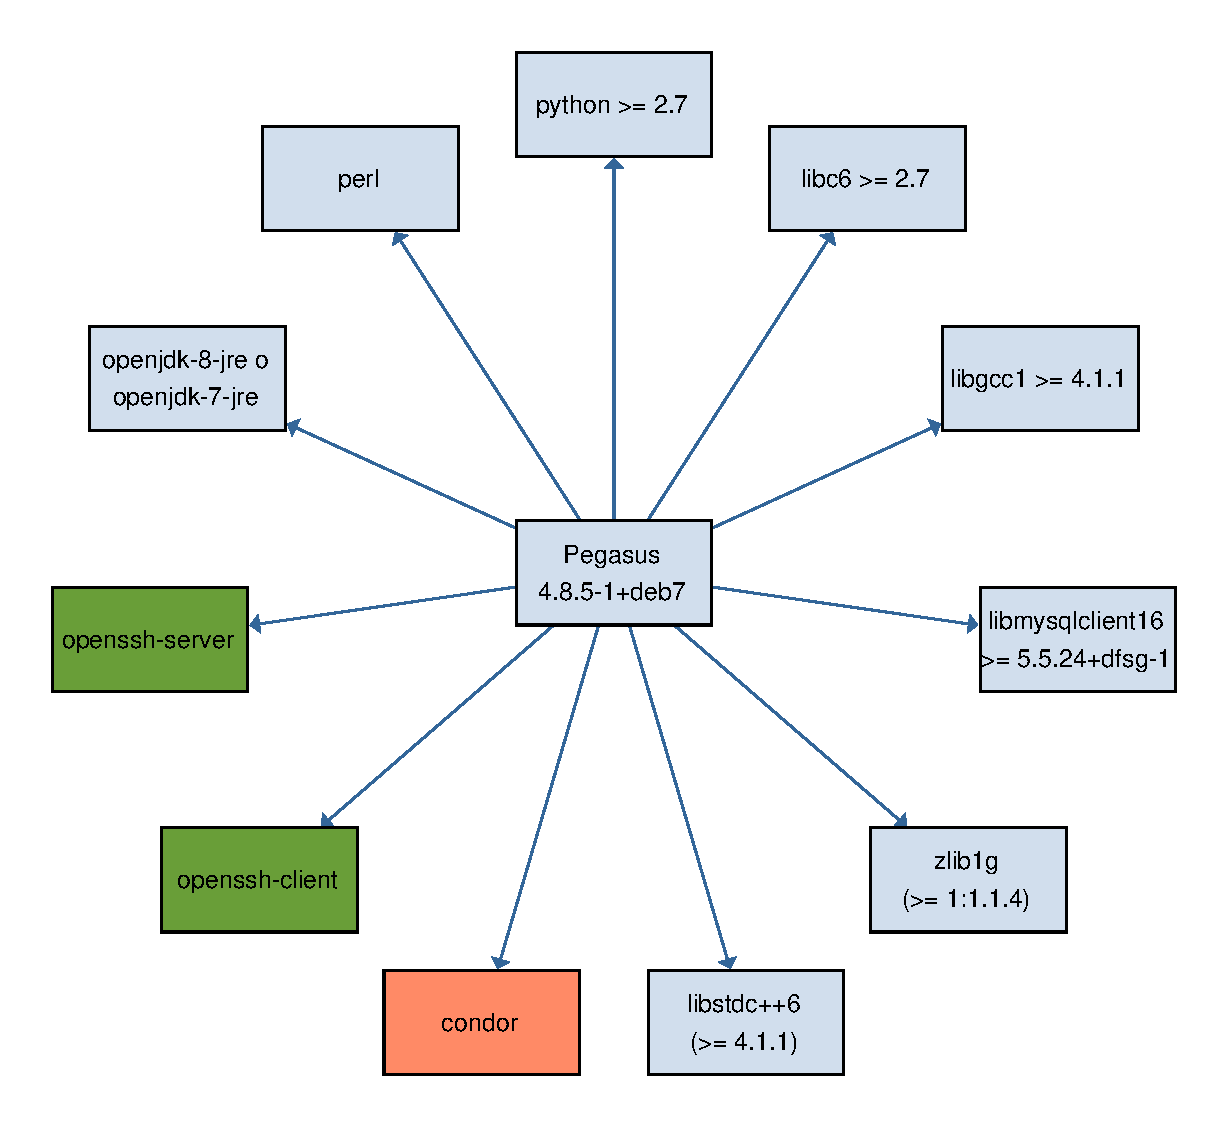
\includegraphics[width=.5\textwidth]{Figures/pegasus-deps}
\caption{Dependencias de Pegasus. En azul: dependencias necesarias y especificadas en el sistema de paquetes. En verde: necesarias pero no especificadas en el sistema de paquetes. En naranjas: dependencias recomendadas}\label{fig:pegasus-deps}
\end{figure}

Las imágenes se encuentran disponibles en DockerHub~\footnote{\url{https://hub.docker.com/r/dockerpedia/pegasus_workflow_images/}}

\subsubsection{Soybean Knowledge Base}

El workflow SoyKB (Soybean Knowledge Base) \cite{joshi2012soybean} permite realizar un proceso de re-secuencia de germoplasma de la soya, ésta ha sido seleccionada para estudiar rasgos como aceites, proteina, resistencia de los nematodos del quiste de la soya y resistencia al estrés.
Pegasus presenta un workflow que implementa polimorfismo de nucleótido único (SNP), la operación insertar/remover (indel) de la base del genoma de un organismo y una análisis utilizando el software GATK \footnote{\url{https://software.broadinstitute.org/gatk/}}
La figura \ref{fig:soykb} muestra   una representación gráfica del workflow, donde se realiza un análisis en paralelo de las muestras para que sean alineadas con el genoma de referencia y se identifique los indels y SNPs. Luego fusiona y filtra los resultados. 

\begin{figure}[t]
\centering
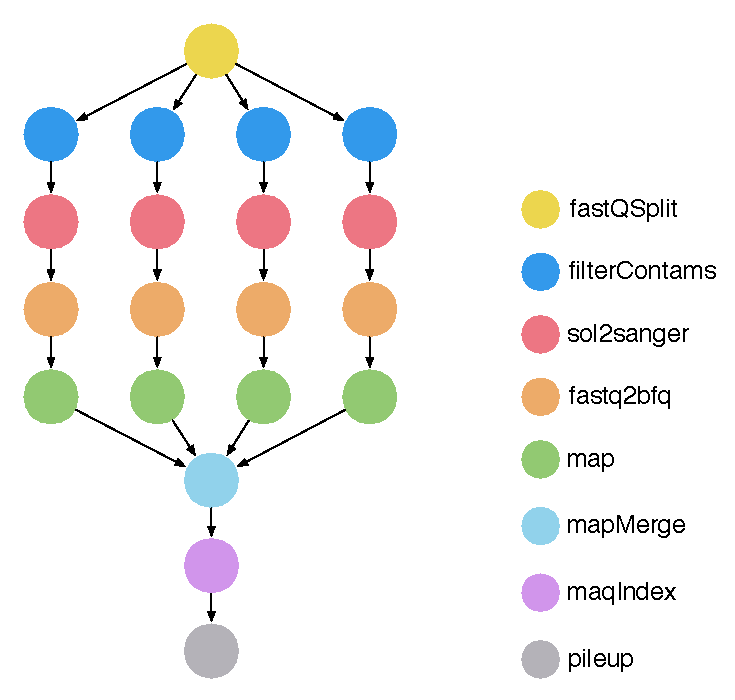
\includegraphics[width=.5\textwidth]{Figures/workflow-genome}
\caption{Representación entregada por Pegasus del workflow SoyKB.}\label{fig:soykb}
\end{figure}

Los componentes de software utilizados por SoyKB se clasifican en dos tipos: propio (en amarillo) y de terceros (en verde). Los componentes principales son: bwa, gatk y bwa y el software de tercero java-1.7.0

\begin{figure}[t]
\centering
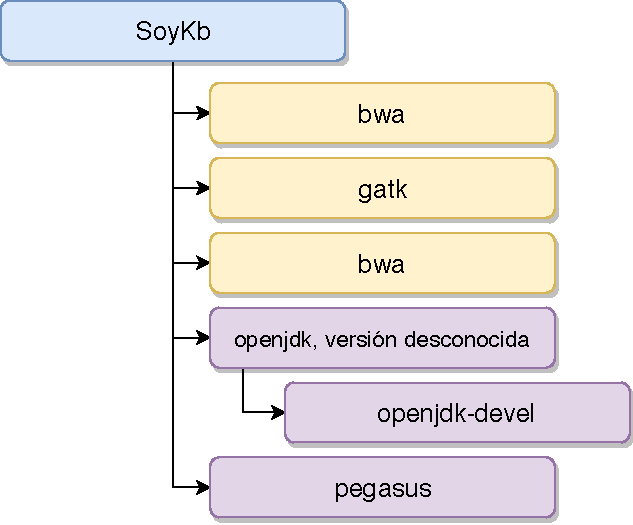
\includegraphics[width=.8\textwidth]{Figures/soykb-deps}
\caption{Dependencias de SoyKb. En amarillo: software propio y en verde software de terceros}\label{fig:modflow} 
\end{figure}

La evaluación de los resultados se realizó de forma manual al igual que en \cite{santana2017reproducibility} debido a los pasos aleatorios del workflow. La metodología fue una verificación manual de la estructura de los resultados, el tamaño de los archivos, número de líneas y la inexistencia de errores.

\subsubsection{Montage}

Montage es un set de herramientas creadas por \textit{NASA Infrared Processing and Analysis Center (IPAC)}, permitiendo generar bajo demanda mosaicos de imágenes astronómicas personalizadas, a partir de archivos de entrada que cumplen con el estándar del Sistema de Transporte Flexible de Imágenes (FITS) y que contienen datos de imágenes registrados en proyecciones que cumplen con los estándares del Sistema Mundial de Coordenadas (WCS).

La figura \ref{fig:montage} entregada por Pegasus ilustra el workflow Montage. Cada uno de los nodos de la figura es un software binario que generan la imagen final.

Debido a que el software es un binario, no se encuentra empaquetado. Por lo tanto fue descargado de la fuente. La dirección de descarga se encuentran en el plan de despliegue \footnote{\url{https://github.com/dockerpedia/montage/blob/master/Dockerfile}}. 

\begin{figure}[t]
\centering
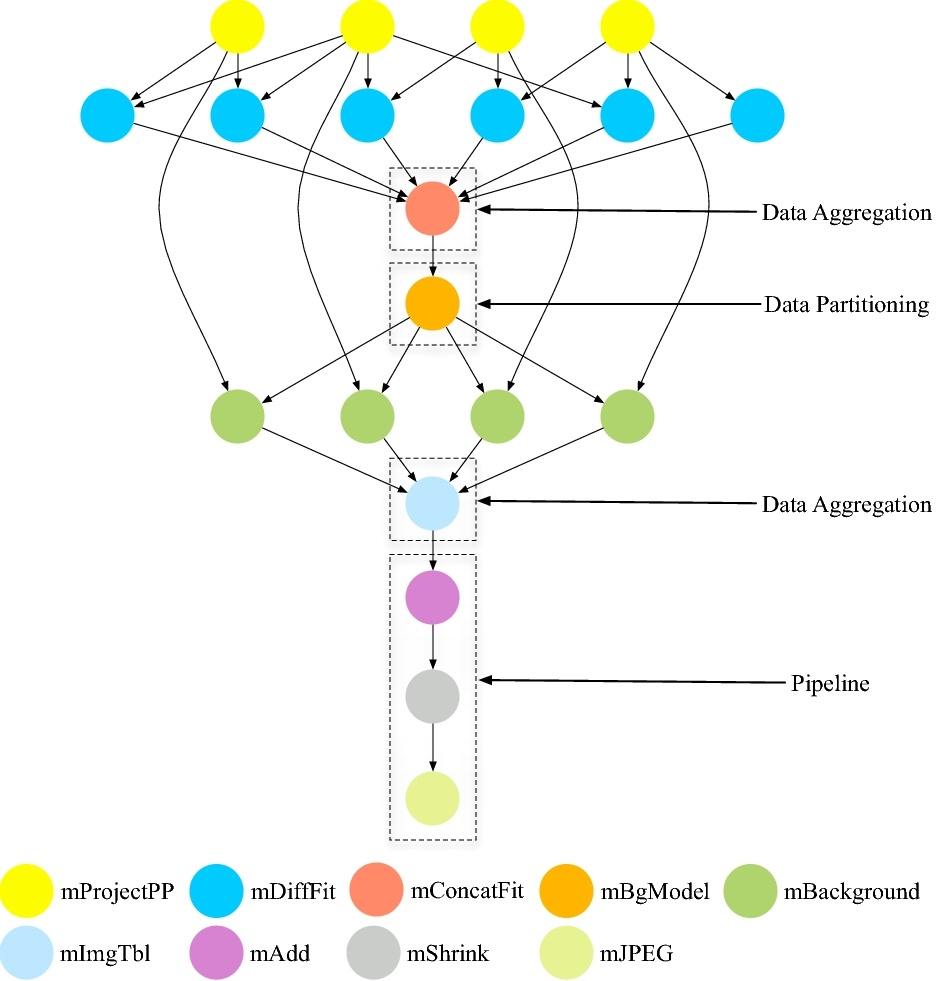
\includegraphics[width=.5\textwidth]{Figures/montage}
\caption{Representación entregada por Pegasus del workflow Montage.}\label{fig:montage}
\end{figure}

En el caso de Montage, se produce una imagen como salida, por ello utilizamos la herramienta de hash perceptual \footnote{\url{http://phash.org}} para realizar la comparación entre la imagen reproducida (imagen del cielo de 0,1 grados) frente a la original.
Como resultado, se obtiene un factor de similitud de 1,0 (más de 1,0) con un umbral de 0,85.
Las figuras \ref{fig:montage-wicus} y \ref{montage-mosorio} muestran las imágenes resultantes y los archivos resultantes en formato FITS se encuentran en nuestro repositorio \footnote{\url{https://github.com/dockerpedia/montage_results}}. 

\begin{figure*}[h]
    \centering
    \begin{subfigure}[b]{0.4\textwidth}
         \centering
         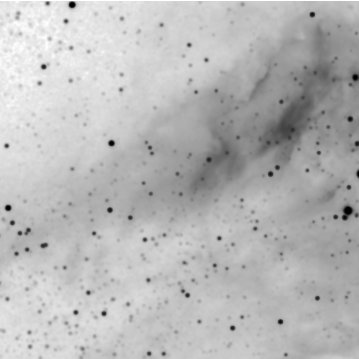
\includegraphics[width=\textwidth]{Figures/montage-original}
         \caption{Resultados originales obtenidos desde WICUS}
         \label{fig:montage-wicus}
     \end{subfigure}
         ~ 
	    \begin{subfigure}[b]{0.4\textwidth}
         \centering
         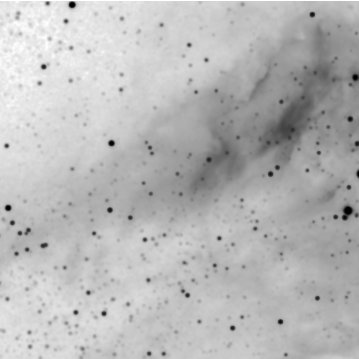
\includegraphics[width=\textwidth]{Figures/montage-mosorio}
         \caption{Resultados reproducidos por nuestra propuesta}
         \label{fig:montage-mosorio}
     \end{subfigure}
        \caption{Los resultados obtenidos con el nuevo ambiente son iguales}
        \label{fig:montage-results}
\end{figure*}



\subsection{dispel4py}

dispel4py ~\cite{} es una biblioteca Python para describir workflow. Describe flujos de trabajo abstractos para aplicaciones intensivas, que luego se traducen y ejecutan en plataformas distribuidas (por ejemplo, Apache Storm, clusters MPI, etc.).
El paquete dispel4py ha sido obtenido del repositorio oficial. Las imágenes están disponibles en DockerHub~\footnote{\url{https://hub.docker.com/r/dockerpedia/internal_extinction/}}. Para la instalación el paquete, utilizamos Conda, un gestor de paquetes, dependencias y entornos para cualquier lenguaje Python, R, Ruby,
Lua, Scala, Java, JavaScript, C/ C\+\+, FORTRAN y es ampliamente utilizado en entornos de \textit{Jupyter notebook}. Para asegurar la versión de los paquetes que se instalarán, incluimos la lista completa de los paquetes instalados en el repositorio GitHub


Los principales requisitos de dispel4py son: python2.7, git y  python-setuptools


Las imágenes se encuentran disponibles en DockerHub~\footnote{\url{https://hub.docker.com/r/dockerpedia//}}



\subsubsection{Internal extinction}

\textit{Internal Extinction of Galaxies} Workflow calcula la extinción interna de galaxias desde el catalogo Amiga. Estos datos son obtenidos a partir de un servicio de Observatorio Virtual, una red de herramientas y servicios que implementan estándares publicados por la \textit{International Virtual Observatory Alliance} (IVOA). El workflow calcula la propiedad, que representa la extinción de polvo dentro de las galaxias y que es un coeficiente de corrección necesario para calcular la luminosidad óptica de una galaxia.

El workflow primero lee el archivo de entregada que contiene la declinación y ascensión recta de 1051 galaxias. Luego, utiliza los valores para realizar consultas al observatorio virtual. Los valores resultantes de las consultas son filtrados seleccionando sólo los valores que correspondan al tipo morfológico (Mtype) y al rango de los ejes del isófito 25 $mag/arcsec^{2}$ (logr25) de las galaxias. Finalmente, se calcula su extinción interna. La figura \ref{fig:internal} muestra los pasos del workflow

\begin{figure}[t]
\centering
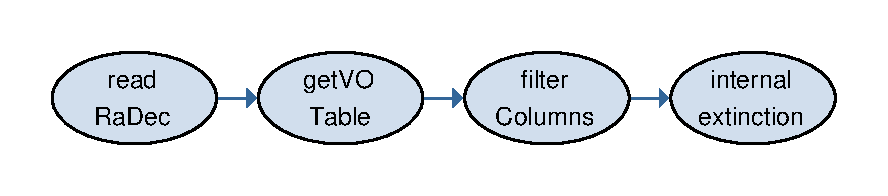
\includegraphics[width=.8\textwidth]{Figures/internal-extinction}
\caption{Pasos necesarios para el workflow internal extinction}\label{fig:internal}
\end{figure}

Nuestra investigación inicial sobre las dependencias para la ejecución de Internal extinction muestra que el software principal requeridos es el siguiente:  \verb|requests==2.20.0|, \verb|python=2.7.15=h33da82c_4|, \verb|numpy=1.15.0=py27h1b885b7_0| y \verb|astropy==2.0.9|


%todo: presentar los resultados




\subsubsection{Seismic Ambient Noise Cross-Correlation}


\textit{Seismic Ambient Noise Cross-Correlation workflow} (o xcorr workflow) es parte del proyecto \textit{Virtual Earthquake and seismology Research Community e-science environment in Europe} (VERCE).
Los terremotos y las erupciones volcánicas en ciertos casos van precedidos o acompañados de cambios en las propiedades geofísicas de la Tierra, como la velocidad de las olas o la velocidad de los eventos. El desarrollo de métodos fiables de evaluación de riesgos para estas amenazas requiere un análisis en tiempo real de los datos sísmicos y un pronóstico verdaderamente prospectivo y pruebas para reducir los sesgos. El objetivo del workflow es la prevision de riesgo a partir del pre procesamiento y correlación de forma cruzada las propiedades anteriores 
xcorr presenta dos etapas, la primera etapa es un preproceso donde cada serie de tiempo continua de una estación sísmica dada (llamada traza), está sujeta a una serie de tratamientos. El procesamiento de cada traza es independiente de otras trazas, haciendo que esta fase sea paralela y la segunda etapa empareja todas las estaciones y calcula la correlación cruzada para cada par. La figura \ref{fig:xcorr} muestra los pasos del workflow.



\begin{figure}[t]
\centering
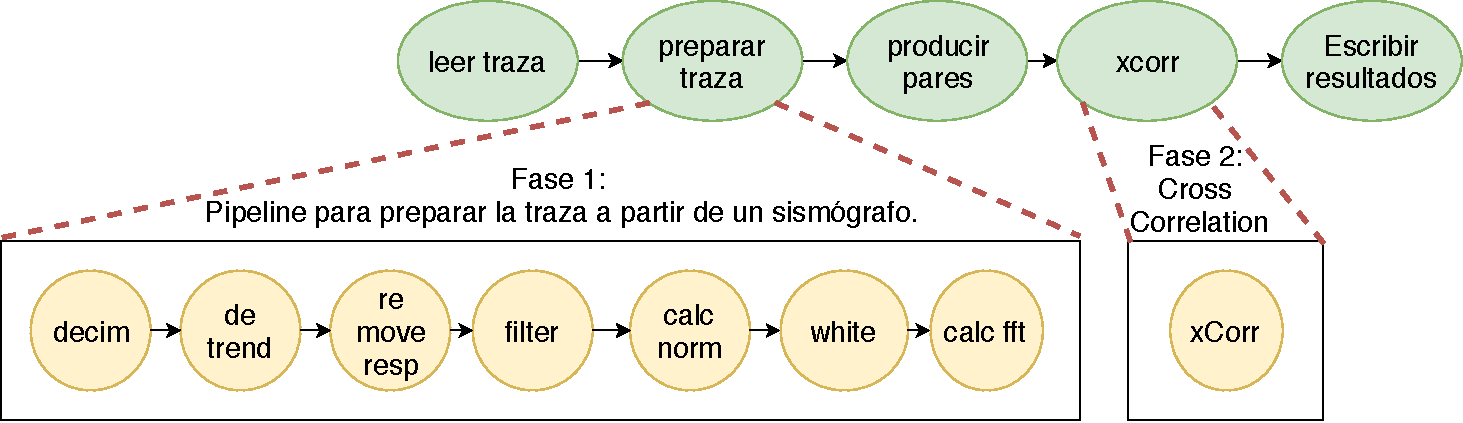
\includegraphics[width=.8\textwidth]{Figures/xcorr}
\caption{Pasos necesarios para el workflow internal extinction}\label{fig:xcorr}
\end{figure}


El software básico para la ejecución de Internal extinction es:  \verb|python=2.7.15=h33da82c_4|, \verb|obspy=1.1.0=py27h39e3cac_2| y \verb|numpy=1.15.0=py27h1b885b7_0|

%todo: presentar los resultados


\subsection{WINGS}

WINGS es un sistema de flujo de trabajo semántico que ayuda a los científicos en el diseño de experimentos computacionales. Un experimento computacional especifica cómo deben ser procesados los conjuntos de datos seleccionados por una serie de componentes de software en una configuración particular.
Los principales requisitos de pegasus son: Docker y Tomcat.
WINGS a diferencia de los otros sistemas de workflows utiliza imágenes Docker para su distribución. La imagen de sistema se encuentra disponible en \footnote{\url{https://hub.docker.com/r/dockerpedia/wings-docker/}}

Los principales requisitos de pegasus son: Java 1.8, Tomcat 8.5, Docker. La figura \ref{fig:pegasus-deps} muestra las dependencias especificadas tanto por el sistema de paquetes o documentación.

\begin{figure}[t]
\centering
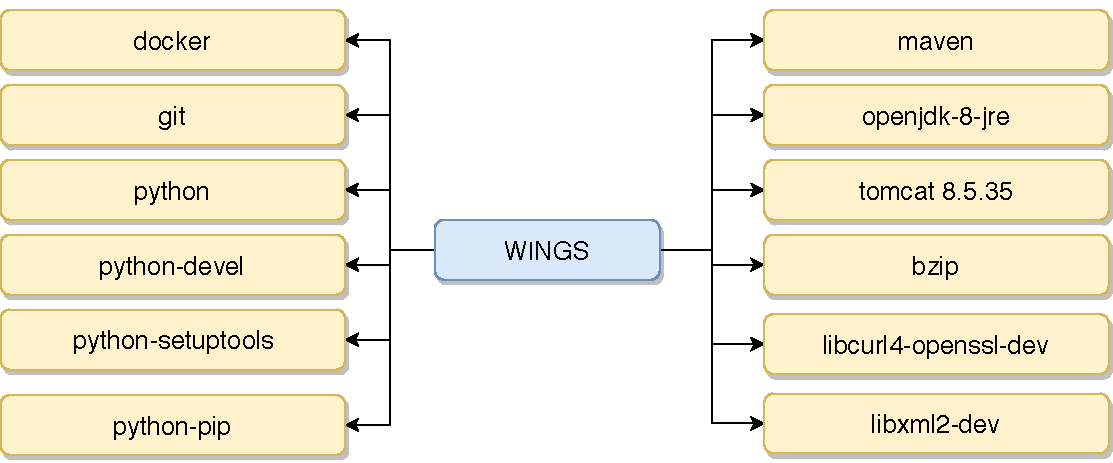
\includegraphics[width=.5\textwidth]{Figures/wings-deps}
\caption{Dependencias de WINGS}\label{fig:wigs-deps}
\end{figure}



Las imágenes se encuentran disponibles en DockerHub~\footnote{\url{https://hub.docker.com/r/dockerpedia/wings/}}


\subsubsection{MODFLOW-NWT}

MODFLOW es el modelo hidrológico modular del \textit{United Satatus Geological Survey} (USGS). MODFLOW se considera una norma internacional para simular y predecir las condiciones de las aguas subterráneas y las interacciones entre las aguas subterráneas y las aguas superficiales.
El USGS MODFLOW-NWT es una formulación de Newton-Raphson para MODFLOW-2005 para mejorar la solución de problemas de flujo de aguas subterráneas no confinadas. MODFLOW-NWT es un programa independiente destinado a resolver problemas de secado y rehumectación de las no linealidades de la ecuación de flujo de agua subterránea no confinada.


\begin{figure}[t]
\centering
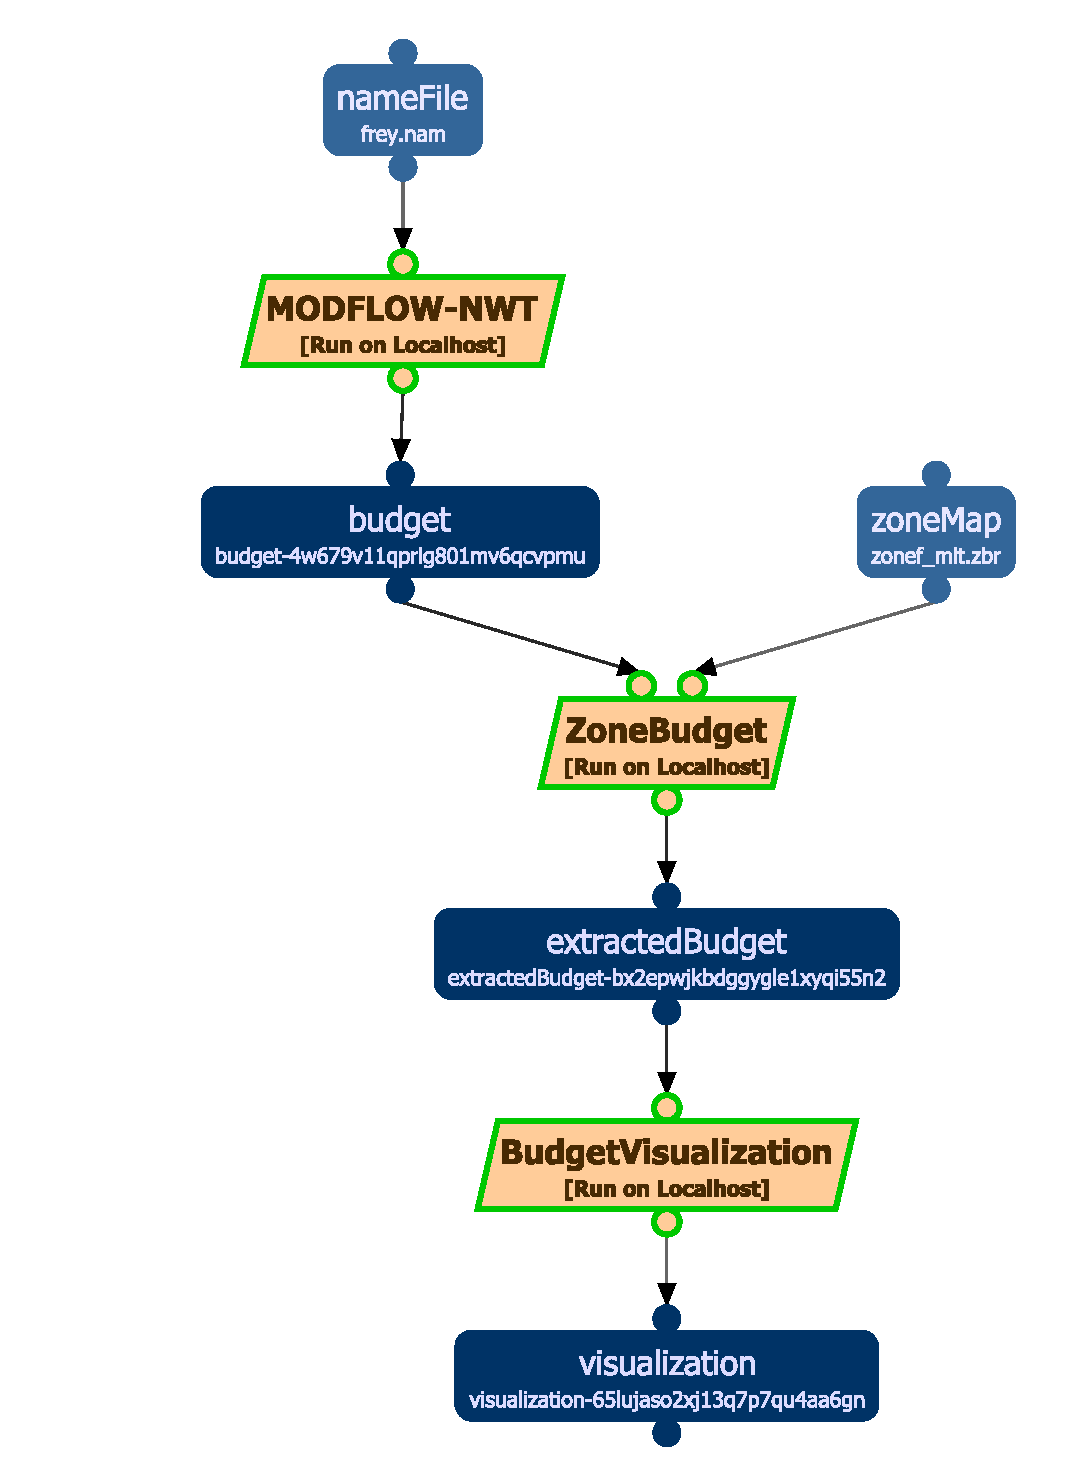
\includegraphics[width=0.6\textwidth]{Figures/usgs-modflow-nwt}
\caption{Figure caption.}\label{fig:modflow}
\end{figure}


La figura \ref{fig:modflow} muestra la estructura principal del worlklow, desarrollado con pipeline compuesto por tres pasos. El proceso inicia leyendo el modelo a utilizar. Luego, el archivo de zona se usa para especificar arreglos de zonas que van usarse y finalmente se genera una visualización que muestra la cantidad de millones de galones por día en zona. Las figuras \ref{fig:modflow-original} y \ref{fig:modflow-reproduced} muestran los resultados generados por el ambiente original y reproducido respectivamente.

\begin{figure*}[]
    \centering
    \begin{subfigure}[b]{\textwidth}
         \centering
         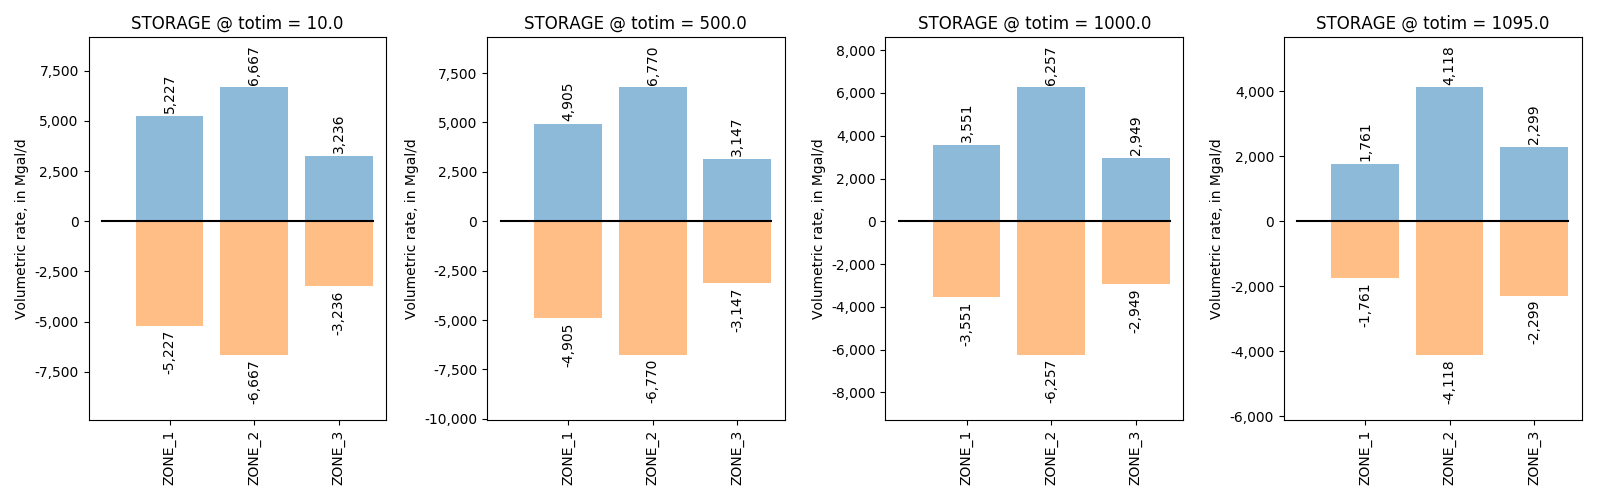
\includegraphics[width=\textwidth]{Figures/viz-original}
         \caption{Resultados originales entregados por el Information Sciences Institute}
         \label{fig:modflow-original}
     \end{subfigure}
	
	    \begin{subfigure}[b]{\textwidth}
         \centering
         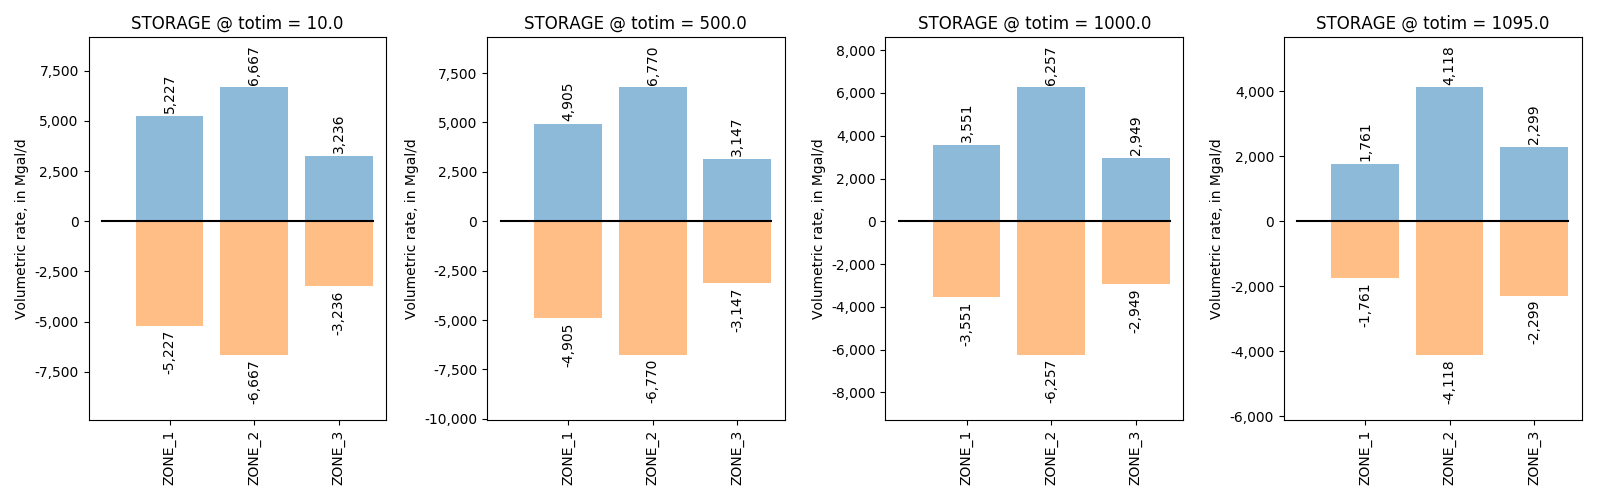
\includegraphics[width=\textwidth]{Figures/viz-reproduced}
         \caption{Resultados reproducidos por nuestra propuesta}
         \label{fig:modflow-reproduced}
     \end{subfigure}
        \caption{Los resultados obtenidos con el nuevo ambiente son iguales}
        \label{fig:both-modflow}
\end{figure*}






%-----------------------------------------------
% 5.2 Physical conservation
%-----------------------------------------------
\section{Conservación física}\label{s5.2}

Dado que publicamos las imágenes con su correspondiente Dockerfile, cualquier usuario puede inspeccionarlas y mejorarlas. Las imágenes puede ser encontradas en DockerHub \footnote{https://hub.docker.com/u/dockerpedia/} y \footnote{\url{https://github.com/dockerpedia}}. 

Para evaluar la conservación física utilizamos tres proveedores diferentes: DigitalOcean, Google Cloud y un local. La figura de \ref{image-env} presenta una descripción de las características de los ambientes    

\begin{table}[]
\centering
\begin{tabular}{|l|l|l|l|}
\hline
Resource   & Digital Ocean & Google Compute & Local     \\ \hline
RAM (GB)   & 8             & 8              & 4         \\ \hline
Disk (GB)  & 100           & 100            & 70        \\ \hline
CPU (GHz)  &               &                &           \\ \hline
CPU (Arch) & 64            & 64             & 64        \\ \hline
OS         & Centos 7      & Debian 9       & Fedora 27 \\ \hline
\end{tabular}
\caption{Image appliances characteristics.}
\label{image-env}
\end{table}

El ambiente debe tener instalado Docker, la información del manifiesto de la imagen de Docker describe la versión de Docker necesaria. Sin embargo, Docker asegura idempontencia para los ambientes CentOS7, Debian 10/9/8/7.7, Fedora 26/27/28, Ubuntu 14.04/16.06/18.04, Windows 10, macOS El Capitan 10.11 o nuevas versiones. El proceso de instalación puede ser encontrado en la documentación oficial \url{https://docs.docker.com/install/}

Cada imagen de Docker tiene archivo README con las instrucciones para correr el experimento. Las figuras \ref{lst:1}~\ref{lst:2} y~\ref{lst:3}  muestran los pasos necesarios para correr el experimento computacional. 

Para correr el experimento y descargar la imagen:

\begin{lstlisting}[caption={Descargar y correr la imagen disponible en DockerHub mosorio/pegasus\_workflow\_images:soykb},label={lst:1},language=bash]
docker run -d --rm -it --name soybean \
 mosorio/pegasus_workflow_images:soykb
\end{lstlisting}

Luego, el usuario debe entrar al container. El usuario puede confirmar que se encuentra dentro del container por el cambio de símbolo de la terminal  (prompt).

\begin{lstlisting}[caption={Entrar al ambiente computacional utilizando bash},label={lst:2},language=bash]
root@docker-instance:~# docker exec \
-ti -u workflow:workflow soybean bash
workflow@a0f861e6fbc4:~ 
\end{lstlisting}

Finalmente, correr el workflow. 

\begin{lstlisting}[caption={Run the workflow},label={lst:3},language=bash]
workflow@a0f861e6fbc4:~/soykb \
./workflow-generator --exec-env distributed	
\end{lstlisting}

Para evaluar si las imágenes Docker son livianas y almacenables, nosotros construimos dos imágenes, una utilizando Docker y otra utilizando máquinas virtuales. La imagen de Docker se construye bajo nuestro enfoque y la imagen de la máquina virtual basada en el trabajo de ~\cite{santana2017reproducibility}. Luego comparamos el uso de disco de ambas.



%-------------------------------------------
% Logical conservation
%-----------------------------------------------
\section{Conservación lógica}\label{s5.3}

A través de las anotaciones realizadas, buscamos describir los ambientes computacionales en forma automática, comparar las diferencias entre dos ambientes y construir un ambiente computacional similar que permita reproducir la ejecución del workflow. 

Para ello, anotamos los flujos de trabajo con nuestra herramienta, las anotaciones están agrupadas por: pasos de construcción y componentes de software. 

Para evaluar la calidad de las anotaciones utilizamos dos experimentos.

\begin{itemize}
	\item Reproducir el ambiente utilizando los pasos de construcción representados por DeploymentPlan
	\item Detectar las similitudes y diferencias entre dos ambientes computacionales usando distintas versiones de la distribución Linux.
\end{itemize}

Para obtener las anotaciones, proponemos usar Clair y construir un sistema de anotador. La figura \ref{fig:arch} muestra los pasos principales del sistema.


\begin{figure*}[]
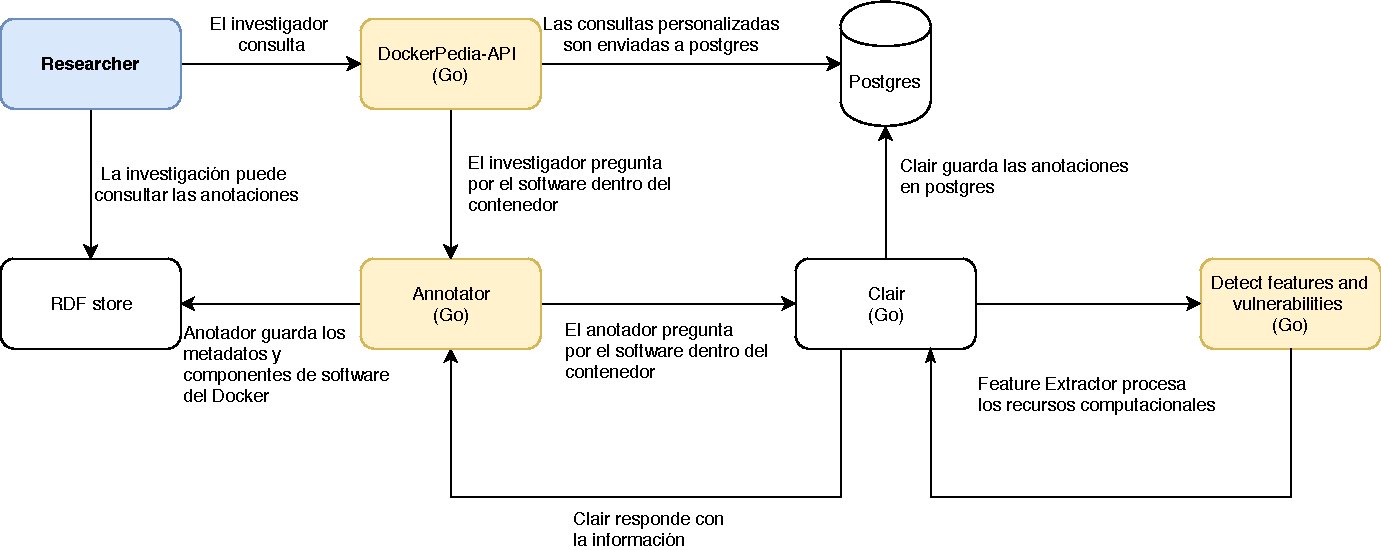
\includegraphics[width=\textwidth]{Figures/arch.pdf}
\caption{Figure caption.}\label{fig:arch}
\end{figure*}


\begin{enumerate}
    \item El investigador pregunta sobre la información de una imagen al sistema anotador. El sistema anotador se encuentra escrito en GoLang y disponible en nuestro repositorio.
    \item El sistema anotador pregunta a Clair sobre software y sus vulnerabilidades de la imagen. Nosotros utilizamos nuestra propia versión de Clair que puede detectar componentes de software instalado por Conda.
    \item Para obtener los pasos de construcción, etiquetas, arquitectura y más información. El anotador obtiene el manifiesto de la imagen desde DockerHub
    \item El sistema anotador guarda la información usando RDF y ontología propuesta.
\end{enumerate}


Para reproducir el entorno, el usuario debe clonar el repositorio y construir la imagen. La URL del repositorio y el cambio asociado (representado por un git commit) se pueden obtener por dos métodos: consultando nuestras anotaciones o usando un comando Docker. El listado \ref{lst:inspect_command} muestra las etiquetas de la imagen de flujo de trabajo SoyKB.


\begin{lstlisting}[caption={Inspect image annotations},label={lst:inspect_command},language=bash]
root@docker-instance:~# docker inspect \ 
    --format='{{json .Config.Labels}}' \ 
    dockerpedia/soykb:latest
\end{lstlisting}

La figura \ref{lst:inspect_result} muestra algunas de las etiquetas de la imagen basado en \textit{Open Container Initiative} 
\begin{lstlisting}[caption={Inspect image annotations},label={lst:inspect_result},language=json]
{
"maintainer": "Maximiliano Osorio <mosorio@inf.utfsm.cl>",
"org.label-schema.build-date": "2018-11-10T21:11:28Z",
"org.label-schema.name": "Soybean Knowledge Base",
"org.label-schema.schema-version": "1.0",
"org.label-schema.url": "http://www.soykb.org/",
"org.label-schema.vcs-ref": "15955b0",
"org.label-schema.vcs-url": "https://github.com/dockerpedia/soykb",
"org.label-schema.vendor": "DockerPedia",
"org.label-schema.version": "1.0"
}

\end{lstlisting}


Para evaluar si los entornos son similares, comparamos ambas imágenes utilizando el lenguaje de consulta SPARQL 1.1. El experimento fue un caso real en el que una imagen podía ejecutar el flujo de trabajo y la otra no. 
La figura \ref{lst:compare_query} muestra la consulta para identificar los diferentes componentes de software entre dos imágenes.

\begin{lstlisting}[caption={¿Cuáles son los diferentes componentes entre dos imágenes?},label={lst:compare_query},language=sparql]
SELECT * WHERE {
 pegasus_workflow_images%3Alatest
  vocab:containsSoftware ?p .
 MINUS{
 pegasus_workflow_images%3Apegasus-4.8.5
  vocab:containsSoftware ?p   
 }
}
\end{lstlisting}

\begin{lstlisting}[caption={¿Cuáles son los componentes que comparten entre dos imágenes?},label={lst:compare_query},language=sparql]
SELECT * WHERE {
 pegasus_workflow_images%3Alatest
      vocab:containsSoftware ?p .
 pegasus_workflow_images%3Apegasus-4.8.5
      vocab:containsSoftware ?p   
    }
    \end{lstlisting}
    
    
\section{Resultados y discusión}\label{s5.4}
Ejecutamos las imágenes sobre sus plataformas correspondientes. Aún mas, los componentes de software de la plataforma y la versión Docker son diferentes. Sin embargo, Docker garantiza que el software siempre funcionará de la misma manera, independientemente de dónde se instale.
Todas las ejecuciones se compararon con la original en una imagen VM predefinida, donde ya existía un entorno de ejecución.
Los resultados muestran que los ambientes de ejecución de contenedores son capaces de ejecutar completamente sus workflow relacionados. Para comprobar que no sólo los flujos de trabajo se ejecutan con éxito, sino también que los resultados son correctos y equivalentes, comprobamos los datos de salida producidos. 

Por otra parte, los resultados experimentales muestran que nuestra propuesta puede detectar automáticamente los componentes del software, las vulnerabilidades relacionadas, los pasos de construcción y los metadatos específicos de los experimentos científicos en forma de imágenes Docker. 
Además, los resultados muestran que es posible extender Clair para anotar a otros gestores de paquetes. 

Las anotaciones generadas por nuestro enfoque permiten comparar los componentes de software entre dos o más entornos. Esta función se puede utilizar como herramienta de depuración cuando un entorno reproducido no funciona.
Por ejemplo, en agosto de 2018, construimos la imagen del workflow SoyKB, y pudimos ejecutar el flujo de trabajo con éxito. Sin embargo, reconstruimos una nueva imagen en noviembre con el mismo DeploymentPlan y no se pudo ejecutar el workflow con éxito.


Describimos los componentes de software dentro de ambas imágenes. Y encontramos las siguientes diferencias:
\begin{itemize}
    \item Agosto: Pegasus 4.8 y Java 1.7
    \item Noviembre: Pegasus 4.9 y Java 1.8
\end{itemize}

Así, analizamos el código y la documentación de SoyKB y las dependencias de Pegasus 4.9. Como resultado, obtuvimos las gráficas de dependencia mostradas en la figura \ref{fig:pegasus49}.  Los gráficos de dependencia muestran que el paquete Pegasus 4.9 y SoyKB no son compatibles debido a sus requerimientos de versión Java.

Así, construimos una nueva imagen instalando Pegasus 4.8, y obtuvimos los gráficos de dependencia que se muestran en la figura \ref{fig:pegasus48}. Aquí, el gráfico no tiene un conflicto y se pudo ejecutar el workflow con éxito.


La nueva imagen fue nombrada como: \verb|pegasus_workflow_images:4.8.5|


\begin{figure*}[]
    \centering
    \begin{subfigure}[b]{0.40\textwidth}
         \centering
         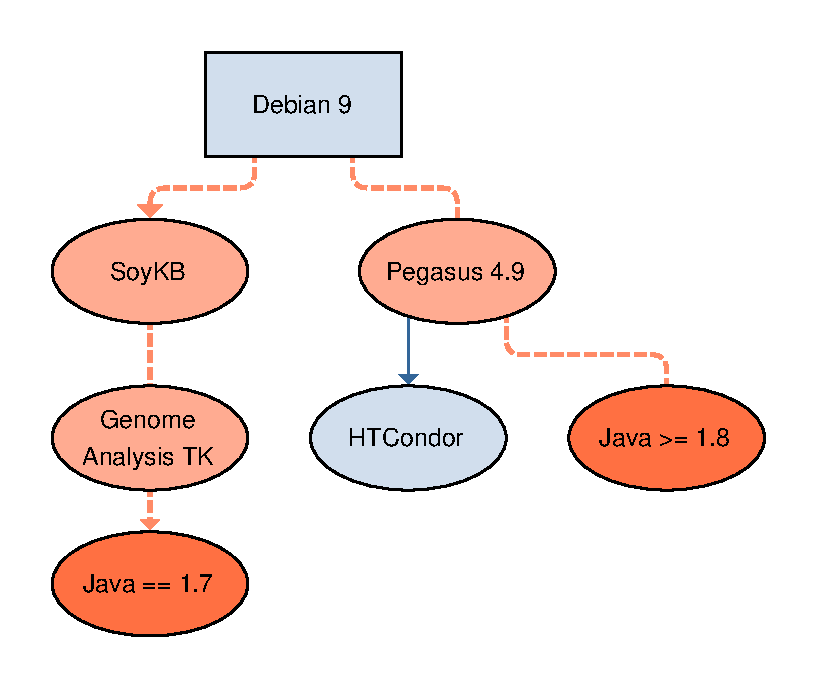
\includegraphics[width=\textwidth]{Figures/pegasus-49.pdf}
         \caption{Dependencies graph Pegasus 4.9 and SoyKB}
         \label{fig:pegasus49}
     \end{subfigure}
    ~ 
    \begin{subfigure}[b]{0.40\textwidth}
         \centering
         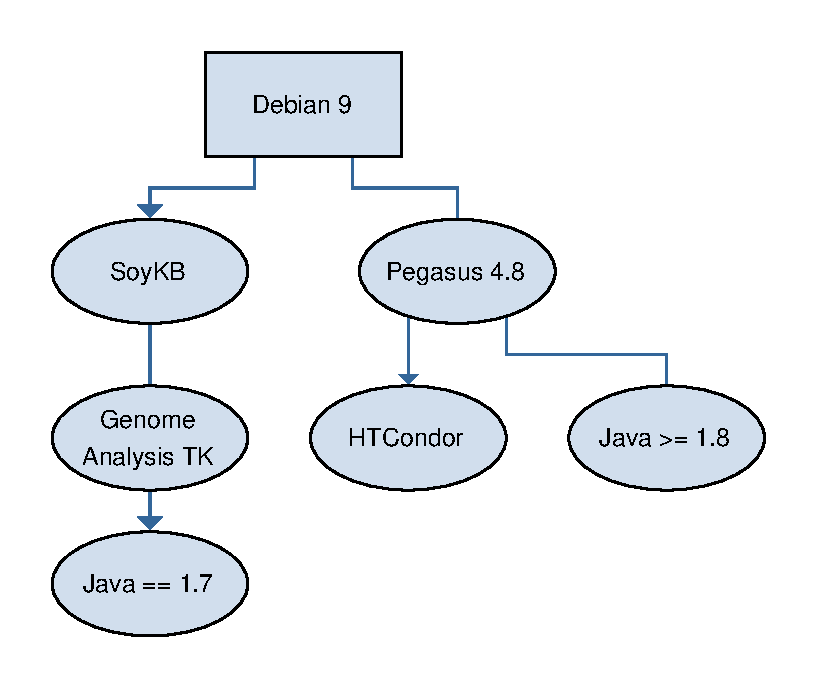
\includegraphics[width=\textwidth]{Figures/pegasus-48.pdf}
         \caption{Dependencies graph Pegasus 4.8 and SoyKB}
         \label{fig:pegasus48}
     \end{subfigure}
        \caption{The orange nodes are the differences between the images}
        \label{fig:dependencies-graph}
\end{figure*}


La razón principal de los trabajos anteriores para evitar la conservación física era la gran demanda de almacenamiento de máquinas virtuales. Afirmamos que las imágenes Docker son ligeras. 

Los resultados de la comparación del uso del disco muestran que hay una disminución del 64,2\% para la imagen Pegasus y del 41,5\% para la dispel4py. La tabla \ref{storage-reduce} muestra la diferencia para el sistema de flujo de trabajo Pegasus y dispel4py.


\begin{table}[]
\centering
\begin{tabular}{|l|l|l|}
\hline
Enfoque        & Pegasus (MB) & dispel4py (MB) \\ \hline
Virtualization & 1929         & 3509 \\ \hline
Container      & 690          & 2500 \\ \hline
\end{tabular}
\caption{Uso de disco de las imágenes pegasus y dispel4py utilizando máquinas virtuales y containers}
\label{storage-reduce}
\end{table} 
% Chapter Template

\chapter{Conclusiones y trabajo futuro} % Main chapter title

\label{ChapterX} % Change X to a consecutive number; for referencing this chapter elsewhere, use \ref{ChapterX}

%----------------------------------------------------------------------------------------
%	SECTION 1
%----------------------------------------------------------------------------------------

\section{Main  1}

m at, molestie in quam. Aenean rhoncus vehicula hendrerit. 
 

%----------------------------------------------------------------------------------------
%	THESIS CONTENT - APPENDICES
%----------------------------------------------------------------------------------------

\appendix % Cue to tell LaTeX that the following "chapters" are Appendices

% Include the appendices of the thesis as separate files from the Appendices folder
% Uncomment the lines as you write the Appendices

% Appendix A

\chapter{Frequently Asked Questions} % Main appendix title

\label{AppendixA} % For referencing this appendix elsewhere, use \ref{AppendixA}

\section{How do I change the colors of links?}

The color of links can be changed to your liking using:

{\small\verb!\hypersetup{urlcolor=red}!}, or

{\small\verb!\hypersetup{citecolor=green}!}, or

{\small\verb!\hypersetup{allcolor=blue}!}.

\noindent If you want to completely hide the links, you can use:

{\small\verb!\hypersetup{allcolors=.}!}, or even better: 

{\small\verb!\hypersetup{hidelinks}!}.

\noindent If you want to have obvious links in the PDF but not the printed text, use:

{\small\verb!\hypersetup{colorlinks=false}!}.

%\include{Appendices/AppendixB}
%\include{Appendices/AppendixC}

%----------------------------------------------------------------------------------------
%	BIBLIOGRAPHY
%----------------------------------------------------------------------------------------

\printbibliography[heading=bibintoc]

%----------------------------------------------------------------------------------------

\end{document}  
